%% Unfolding and respective studies
\section{Correcting for detector effects}
\label{sec:unfolding}

When an observable is measured by a particle physics experiment, it is important to note that the measured distribution, (i.e. what the particle detector sees) is not what truly occurs at the particle-level. Rather, it is a convolution of the underlying physics process with the effects of the detector. The \ATLAS detector, although an astonishing feat of technology, is still subject to resolution, acceptance, and efficiency limitations. The data at the detector level is smeared and includes the effects of these limitations. For an inclusive measurement such as the four-lepton invariant mass distribution, it is often desirable to correct for these detector effects and present the data at the particle-level. In high energy physics, the term coined for this correction procedure is unfolding. Unfolding measurements and presenting them at the particle level has many advantages. In doing so, the measurement may be directly compared to theoretical predictions, as well as particle-level results from other experiments, in the years to come. Furthermore, they can be rapidly compared to newly available BSM simulations in re-interpretation studies. The concept of re-interpretation is further explored in Chapter~\ref{chap:reinterpretation}. 

\subsection{Unfolding methodology}
\label{subsec:unfmethod}

Unfolding in particle physics can be more generally referred to as a deconvolution. The generic problem statement of deconvolution is to derive a relationship between the true distribution $T(x)$ and the recorded distribution $D(y)$. The two are related by a smearing function $R(x,y)$, which encompasses the instrumentation effects in making the measurement. 
\begin{equation} \label{eq:unfintegral}
    T(x)=\int S(x,y)D(y)dy
\end{equation}
Due to the discretised nature of histograms, the unfolding problem can be stated as a matrix equation:
\begin{equation} \label{eq:unfmatrix}
    x_i=S_{ij}y_j
\end{equation}
where $R$ represents the a smearing matrix of sorts, \todo{add more}$T$ is the true histogram at particle-level, and $D$ is the reconstructed histogram at detector-level. 

For the four-lepton invariant mass analysis, an iterative unfolding method motivated by Bayesian statistics, popularised by Giulio D’Agostini, is chosen. The method iteratively applies the three inputs described above to the measured distributions while using the particle-level SM prediction as a prior.

\subsubsection{An iterative Bayesian approach to unfolding}
\label{ssec:bayesianunfolding}
Let there be a set of causes $C_i$, that can produce one effect $E$. 
\begin{equation}
    P(C_i|E)=\dfrac{P(E|C_i)\cdot P(C_i)}{\Sigma_{k=1}P(E|C_k)\cdot P(C_k)}
\end{equation}

\begin{itemize}
    \item $P(C_i|E)$: given the effect, the conditional probability that it was produced from the $i$-th cause.
    \item $P(E|C_i)$: for the $i$-th cause, the conditional probability that the effect is produced.
    \item $P(C_i)$ is the initial probability of the $i$-th cause.
\end{itemize}
If there are multiple possible effects for the causes, then the formula can be generalized to be:
\begin{equation}
    P(C_i|E_j)=\dfrac{P(E_j|C_i)\cdot P(C_i)}{\sum_{k=1}P(E_j|C_k)\cdot P(C_k)}
\end{equation}
The number of expected events for each cause $C_i$ can be obtained by multiplying the number of observations made for effect $j$ with the probability it had been due to cause $i$, and summing over all effects:
\begin{equation} \label{eq:numcause}
    N(C_i)=\sum_jN(E_j)\cdot P(C_i|E_j).
\end{equation}
Here a parallel can be drawn back to equation \ref{eq:unfmatrix}, where $N(C)={N(C_1),N(C_2),...,N(C_n)}$ represents the number of events in the $n$ bins of the true histogram $x_i$, and $P(C_i|E_j)$ corresponds to $R$. Combining these equations, the procedure for estimating the true histogram can be written as:
\begin{equation}\label{eq:bayesianunfolding}
    x_i=\sum_{j=1}^n\dfrac{R_{ij}\cdot P(x_i)}{\sum_{k=1}^nR_{kj}\cdot P(x_k)}y_j.
\end{equation}
Here the matrix defined as $R_{ij}$ is the called the response matrix. The denominator in the equation is a normalization factor using the y-projection of the matrix. $P(x_i)$ is the prior, which is updated in each iteration with the unfolded true distribution $x_i$, also known as the posterior.
\todo[inline]{Perhaps mention other unfolding methods and justify choice of this one?}

\subsection{Unfolding inputs}
Below is a summary of the terminology commonly used inputs in the unfolding procedure. These inputs are generated using the Monte Carlo simulations described in Section~\ref{sec:montecarlopred}. 

\begin{itemize}
    \item Fiducial fraction $f_i$: this is a one-dimensional correction that accounts for events which do not enter into the fiducial region, but pass the detector-level selection nonetheless. These occur due to the finite resolution in the measurement the variables used to select events. The fiducial fraction is defined as the ratio of events that pass both fiducial and detector-level selection to events that pass detector-level selection only.
    \item Reconstruction efficiency $\epsilon_i$: this accounts for the acceptance and efficiency of the detector in reconstructing an event. Of all the events that pass the fiducial selection, only a fraction will be successfully reconstructed and visible to the detector. Formally the reconstruction efficiency is also a one-dimensional correction; defined as the ratio of events which pass both the fiducial and detector-level selection to events that pass fiducial-level selection only.
    \item Migration matrix $M_{ij}$: each bin in the histogram of the measured observable represents a sub-range of observable values. Sometimes the detector may smear the observable's value high or low enough such that it gets filled to different bins in particle-level and detector-level. These are referred to as bin-to-bin migrations, and is corrected for by the migration matrix. This is constructed as a two-dimensional matrix using events which pass both fiducial and detector-level selection, with the value at particle-level on one axis and the value at detector-level on the other. The matrix, $M_{ij}$, represents the probability that an event which falls into bin $i$ at particle-level will fall into bin $j$ when reconstructed at the detector-level. The diagonal elements of the migration matrix is defined as the unfolding stability; the fraction of events in a particle-level bin which are reconstructed in same bin at detector level.
    \item Fiducial purity: similar to the unfolding stability, but not the same. The fiducial purity accounts for the probability that an event in the detector-level bin $i$ originated from the same particle-level bin $i$. 
\end{itemize}

The construction of the response matrix $R_{ij}$ is done using the above inputs. It is defined as:
\begin{equation}
    R_{ij} = M_{ij}\epsilon_jf_i.
\end{equation}
The unfolding software used for this analysis (VIPUnfolding) takes the migration matrix, reconstruction efficiency, and fiducial fraction as inputs, and constructs the response matrix within the software. 

Figure~\ref{fig:inclm4lunf} shows the unfolding inputs for the inclusive \mFourL{} distribution. In the left panel there are the detector-level and particle-level yields, and in the right panel the fiducial fraction, reconstruction efficiency, and fiducial purity are plotted. The inputs here include the application of the pre-unfolding weight (see Section~\ref{subsec:preuf}). The event count on the $y-$axis shows events per bin and serves as a visual check to ensure all bins have fourteen or more events. The fiducial purity in yellow, likewise, should always be above 0.6. The purity tends to be lower in the middle mass range and around the $Z$ and Higgs peaks due to narrow bin widths. The fiducial fraction in blue is above 85\% in all bins, levelling out to 95\% for $\mFourL{} > 200$~\GeV. The efficiency in red is lowest below 80\% for the first two mass bins, due to the higher inefficiency when reconstruction low mass electrons and muons. 

 The residual efficiency correction taking into account the pre-unfolding weights and the fiducial fraction for the full fiducial phase-space as well as for each of the four $\mFourL$ slices are shown in Table~\ref{tab:fidxsunf}.
 In order to illustrate the effect of the pre-unfolding and to show what the size of corrections would be if pre-unfolding were not applied, Tabe~\ref{tab:fidxsunf-nopreunfold} shows the efficiency corrections and fiducial fractions before pre-unfolding.
 \begin{table}[ht]
     \centering
     \begin{tabular} { c | r@{$\pm$} l  r@{$\pm$}l }
       \hline
       Region & \multicolumn{2}{c}{Eff. correction}  & \multicolumn{2}{c}{Fid. fraction}   \\
       \hline
       Full fid. phase-space & $0.879$ & $0.021$ & $0.9521$ & $0.0033$ \\[0.3cm]
       $Z\to 4\ell$ region  & $0.79$ & $0.04$ & $0.914$ & $0.009$ \\
       $H\to 4\ell$ region  & $0.898$ & $0.028$ & $0.937$ & $0.005$ \\
       Off-shell region & $0.842$ & $0.028$ & $0.919$ & $0.006$ \\
       On-shell region  & $0.930$ & $0.012$ & $0.9754$ & $0.0017$ \\
       \hline
    \end{tabular}
   \caption{Efficiency correction taking into account the pre-unfolding weights and fiducial fraction for the full fiducial phase space and the $\mFourL$ slices. The quoted uncertainties take into account the full set of systematics discussed in Section~\ref{sec:uncertainties} \label{tab:fidxsunf} }
 \end{table}

 \begin{table}[ht]
     \centering
     \begin{tabular} { c | r@{$\pm$} l  r@{$\pm$}l }
      \hline
     Region & \multicolumn{2}{c}{Eff. correction}  & \multicolumn{2}{c}{Fid. fraction}   \\
       \hline
    %   Full fid. phase-space & $0.879$ & $0.021$ & $0.9521$ & $0.0033$ \\[0.3cm]
       $Z\to 4\ell$ region  & $0.425$ & $0.019$ & $0.930$ & $0.009$ \\
       $H\to 4\ell$ region  & $0.534$ & $0.017$ & $0.948$ & $0.005$ \\
       Off-shell region & $0.498$ & $0.017$ & $0.934$ & $0.006$ \\
       On-shell region  & $0.677$ & $0.009$ & $0.978$ & $0.002$ \\
       \hline
    \end{tabular}
   \caption{Efficiency correction and fiducial fraction for the full fiducial phase space and the $\mFourL$ slices, without the pre-unfolding weights applied. The quoted uncertainties take into account the full set of systematics discussed in Section~\ref{sec:uncertainties} \label{tab:fidxsunf-nopreunfold} }
 \end{table}

Figure~\ref{fig:inclm4lmat} shows the migration matrix for the inclusive \mFourL{} distribution. The $x-$axis has the detector-level bins, the $y-$axis has the particle-level bins, and the matrix is normalized to the $y-$axis. The numbers in each square is the percentage probability that an event in particle-level bin $i$ ends up in detector bin $j$. The migration matrix of Figure~\ref{fig:inclm4lmat} is very diagonal. This is a desirable trait in unfolding, as it means the distribution has relatively low amounts of bin-to-bin migrations. Most of the bin migrations are contained within the two neighbouring bins on either of the bin edge.  Similarly in Figure~\ref{fig:inclvm4lmat} there is the migration matrix of the four mass regions dominated by single Z, Higgs,  off-shell ZZ, and on-shell ZZ, in that order. Here the migrations are highest for the off-shell mass slice. This is an expected effect since the off-shell slice consists of three discontinuous mass regions that neighbour all of the three other mass slices. 

The remaining plots of the unfolding inputs and migration matrices for all other observables are available in Appendix~\ref{app:moreunf}.

%%incl.m4l
\begin{figure}[tbh!]
    \begin{subfigure}{.99\textwidth}\centering
      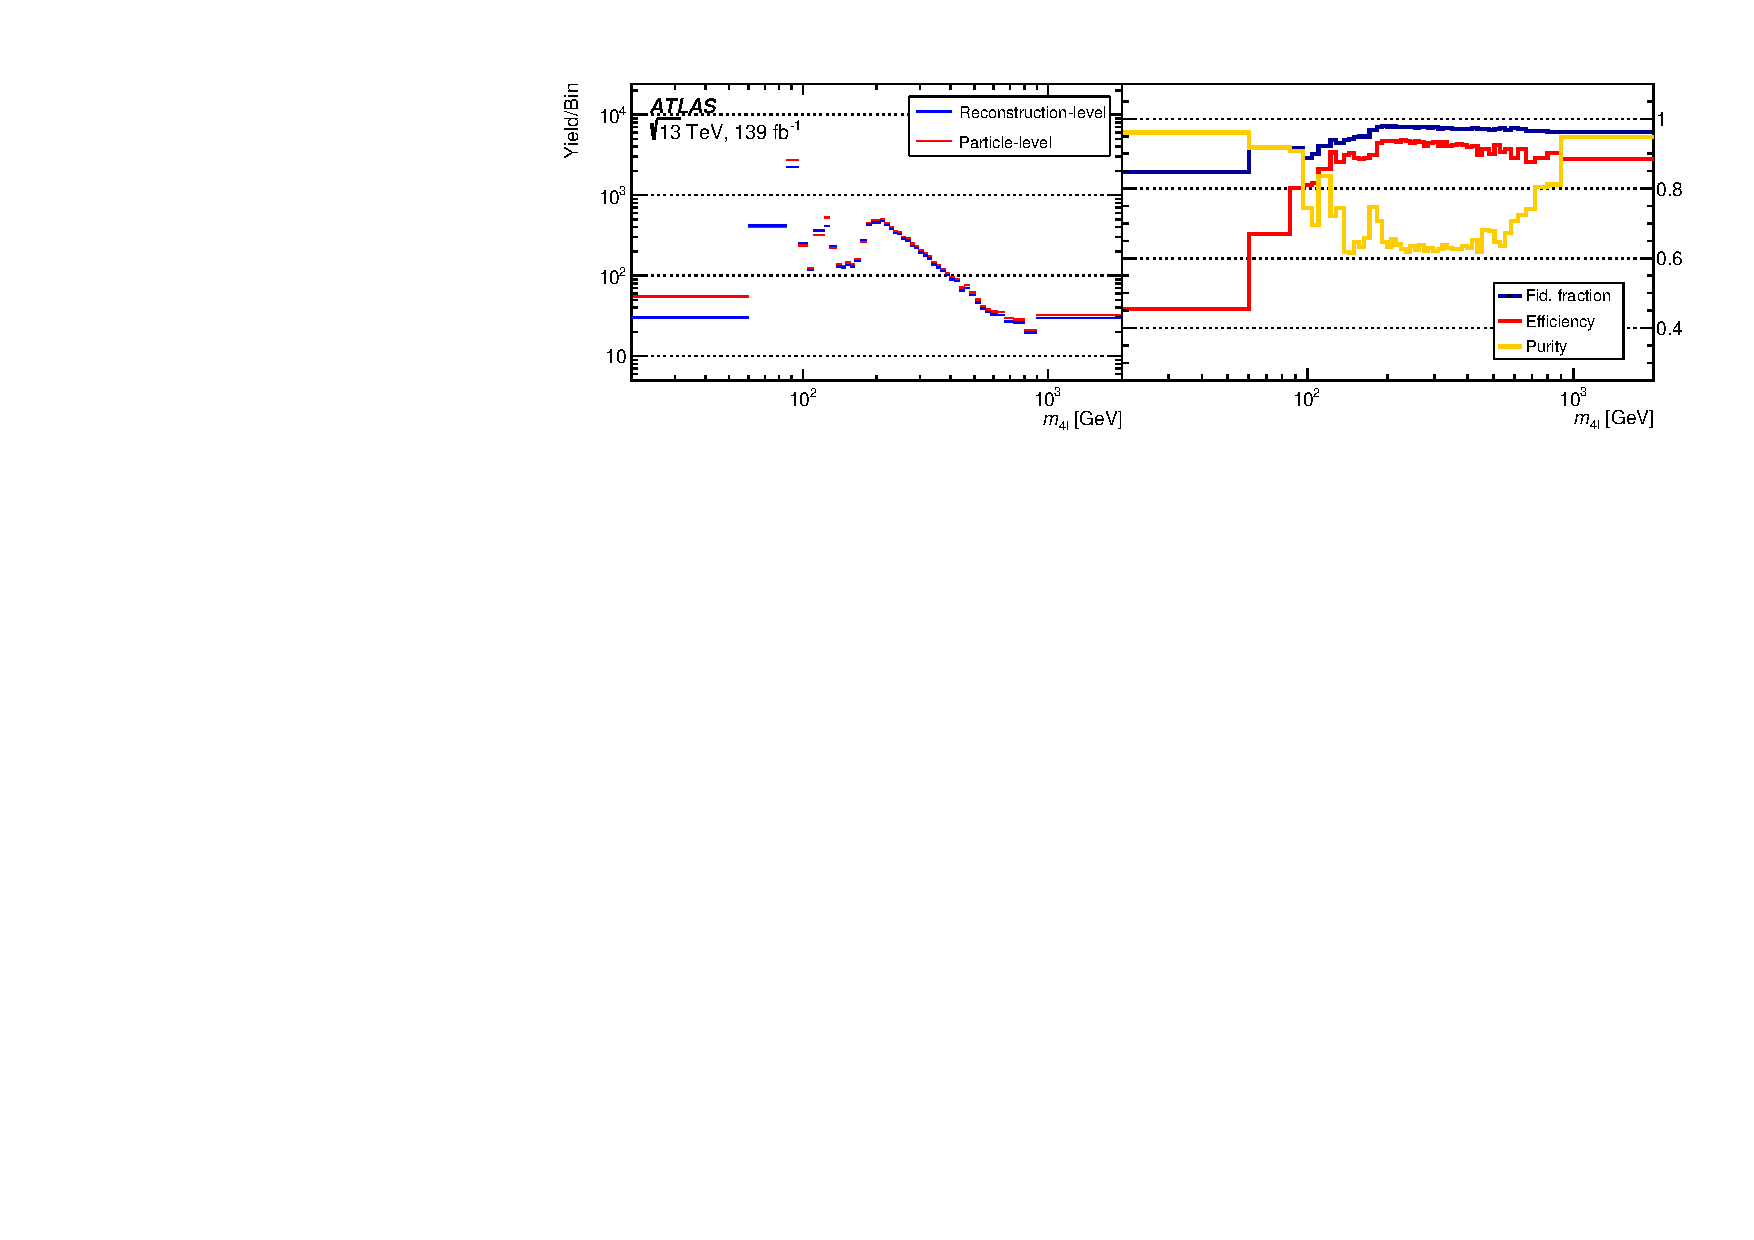
\includegraphics[width=.99\linewidth]{Figures/m4l/UnfoldingStudies/v014_inputs/inclm4linputs.pdf}  
    \end{subfigure}
    \caption{In the left-hand panel, the number of predicted events passing the reconstruction- and fiducial- level selections are displayed as the detector yield and particle yield, respectively. They are given as a function of inclusive \mFourL{} bins. The right-hand panel shows the efficiency, fiducial purity and fiducial fraction in each of the same \mFourL{} bins.}
    \label{fig:inclm4lunf}
\end{figure}
\begin{figure}[tbh!]
  \centering
  \begin{subfigure}{.99\textwidth}\centering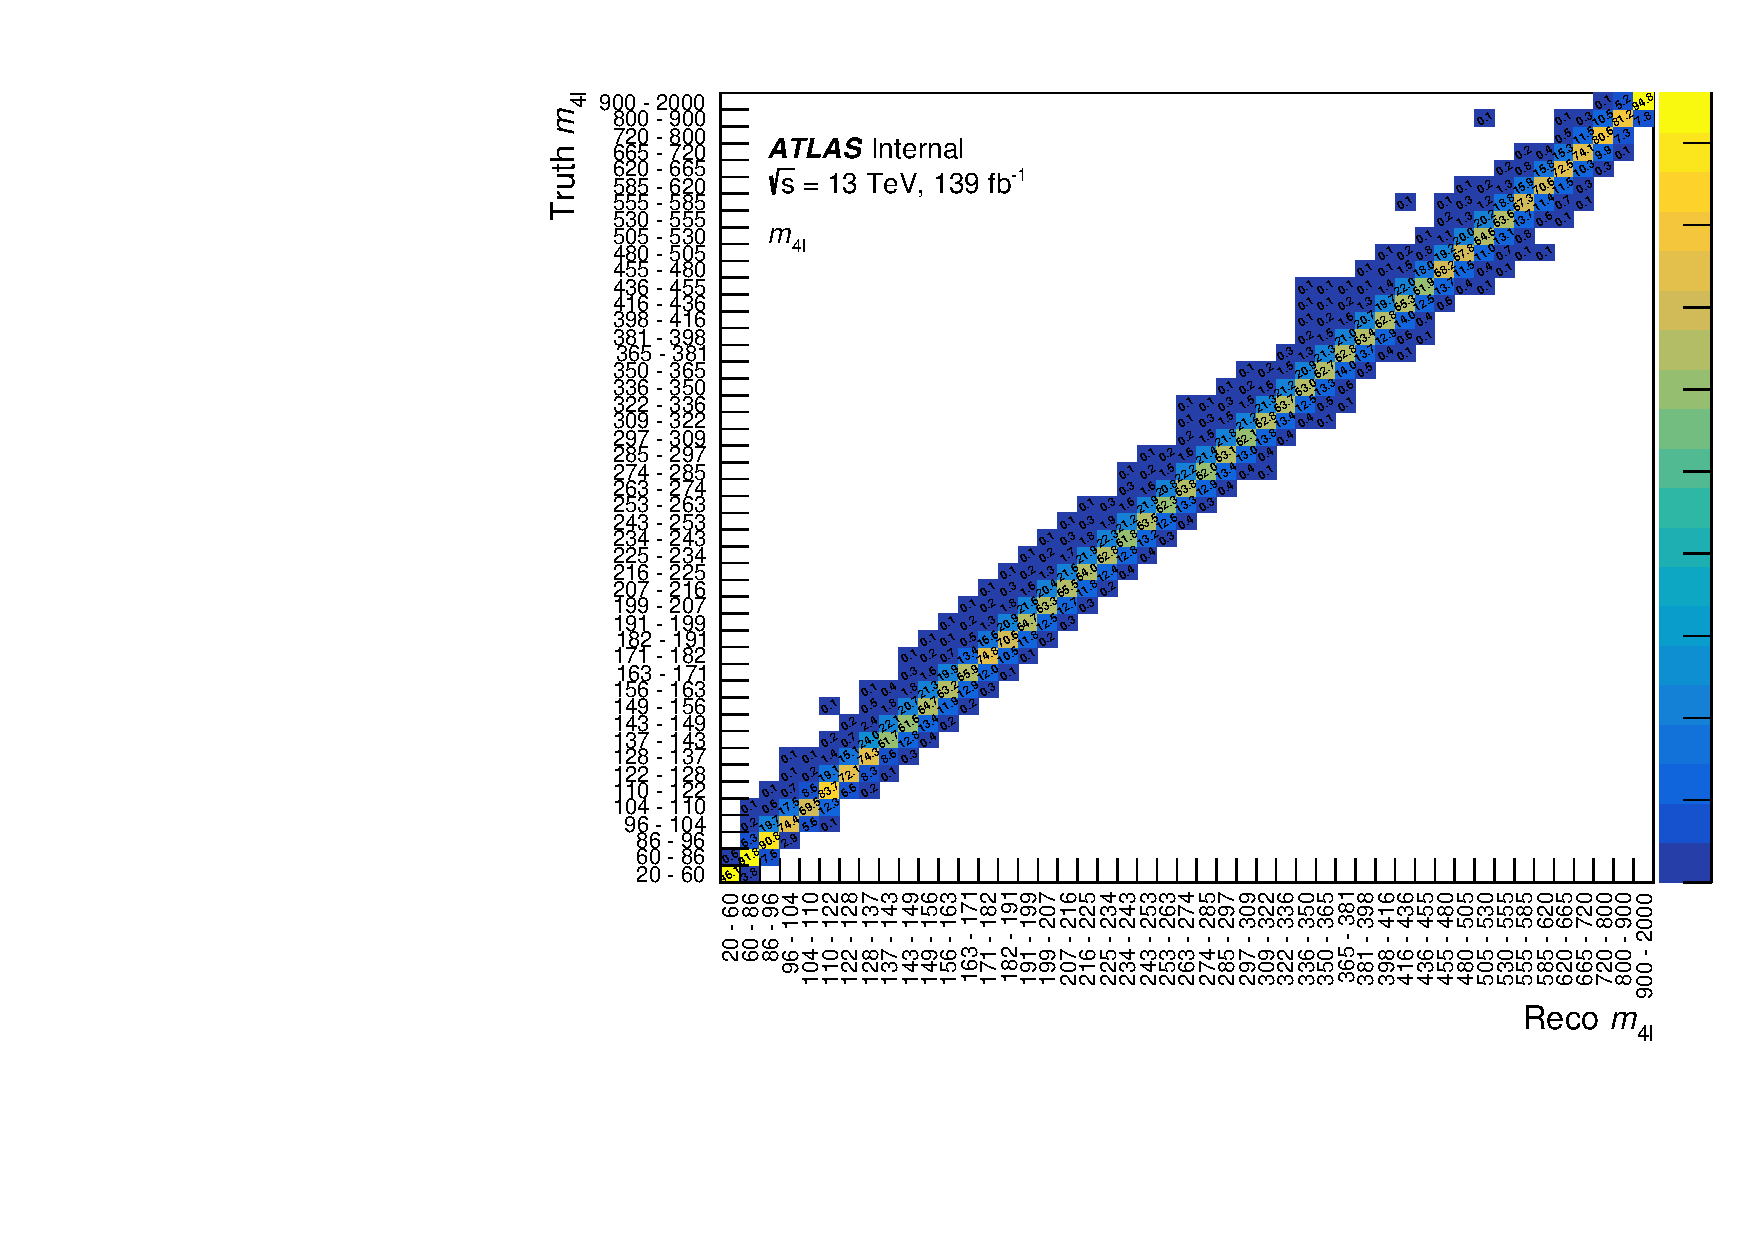
\includegraphics[width = 0.99\textwidth]{Figures/m4l/UnfoldingStudies/v014_matrices/inclm4lMatrix.pdf}\end{subfigure}
 \caption{Migration matrix for the inclusive \mFourL{} distribution. \label{fig:inclm4lmat}}
\end{figure}
\begin{figure}[tbh!]
  \centering
  \begin{subfigure}{.85\textwidth}\centering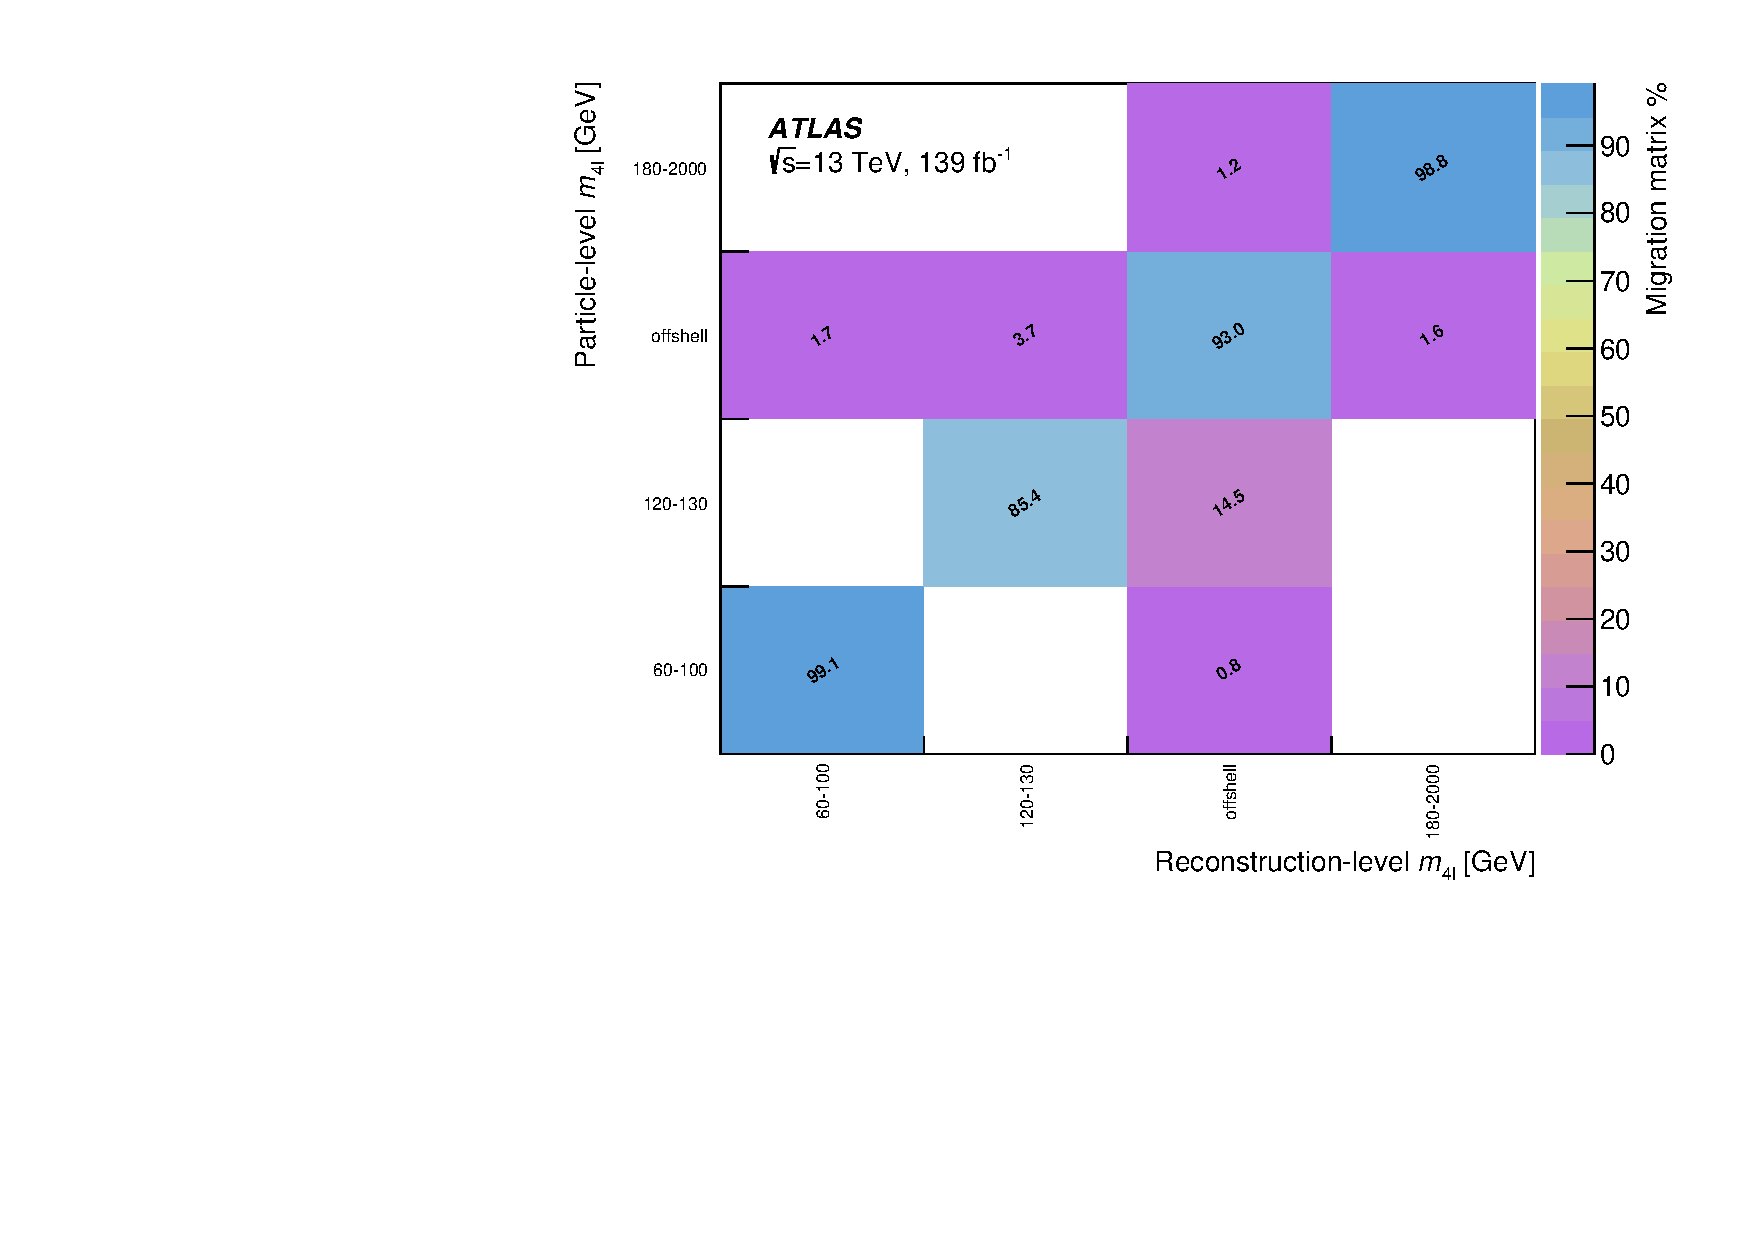
\includegraphics[width = 0.99\textwidth]{Figures/m4l/UnfoldingStudies/v014_matrices/inclusive_vs_m4lMatrix.pdf}\end{subfigure}
 \caption{Migration matrices for the four \mFourL{} regions between the slices. \label{fig:inclvm4lmat}}
\end{figure}

\subsubsection{Number of Bayesian iterations}

When using the iterative Bayesian method to unfold, the number iterations performed is a key parameter and must be optimized. The method, which uses the nominal MC distribution as an initial prior, results in a bias towards the original shape of the nominal prediction. A way to minimize this effect is to use the obtained unfolded distribution from the previous iteration as the prior for the subsequent unfolding iteration. The more iterations there are, the less dependence there is on the prior, and therefore the smaller the bias. A side effect, however, is that increasing the number of iterations also increases the statistical uncertainty. Fluctuations caused by limited statistics become amplified by the feedback in the algorithm. These effects are thoroughly studied in order to strike a balance between minimizing the bias at the cost of increasing the statistical uncertainties.

One thousand toy distributions are generated using the detector-level Standard Model prediction where the value of each bin is randomly drawn from a Gaussian distribution. Each toy is unfolded following the procedure outlined in section \ref{ssec:bayesianunfolding}, where the nominal SM predictions are used to construct the response matrix and for the prior. The bias, written as
\begin{equation} \label{eq:unfbias}
    \text{Bias}_i=\dfrac{\sum_{j=1}^nM_{ij}\cdot x_j-y_i\cdot f_i}{y_i\cdot f_i},
\end{equation}
measures the difference between the product of the migration matrix and the unfolding output, and the product of the detector-level toy and the fiducial fraction. It is an assessment of the strength of the pull that the shape of the SM prior has on the unfolded toy result \todo{Read more about regularization}. Additional, a statistical uncertainty from the unfolding procedure for each individual toy in each bin is quoted. Next, the bias significance\change[]{italics?} per bin is defined as the quotient of the bias and the statistical uncertainty. After sampling over all toys, the root-mean-square (rms) of the bias significance in each bin is calculated. Through the rms bias significance, the size of the bias in comparison to that of the statistical uncertainty is quantified and used as a criterion in determining the number of iterations. The requirement is to use the minimum the number of iterations needed for a bias significant lower than 0.5.

For the inclusive \mFourL{} distribution, the minimum number of iterations for which the criterion is met is three. For the majority of the other measured distributions, three iterations of the unfolding are also found to be optimal. Two iterations are found to be sufficient for the following observables: \mZOne-\mFourL, \dPhill-\mFourL, and \dYPairs-\mFourL.

\subsection{Binning optimization}
\label{subsec:binningopt}

The binnings of the measured distributions were optimized based on two factors: the number of events and the purity of each bin. Here the purity refers to the diagonal of the migration matrix normalised along truth, thus representing the fraction of truth events that end up in the same reconstructed event bin. 

The first iteration of the binnings were run with the nominal criteria. Here, depending on the number of events in the bin, the purity requirement varies. Bins with lower statistics have a high purity requirement to reduce bin-to-bin migrations. The minimum number of events required for each bin is 14. Between 14 and 20 events, the purity was required to be at least 80\%. Between 20 and 25 events the purity must be 70\% or higher. Finally for the higher statistics bins with more than 25 events the purity cut was 60\%. 

The binning algorithm is as follows. For the full \mFourL{} differential mass distribution from \unit{20}{\Gev} - \unit{2000}{\GeV}, the distribution is first split into very fine steps of \unit{1}{\GeV} bins from \unit{20}{\Gev}-\unit{450}{\GeV}. From \unit{450}{\Gev}-\unit{2000}{\GeV} wider steps of \unit{5}{\GeV} bins were used. Due to the fine nature of the bin widths, this initial binning failed to meet any of the binning criteria. Next, the binning algorithm starts from the low mass end and starts to merge adjacent bins together if the criteria were not met. For example, if bin number 1 [20,21]~\GeV has > 10 events, the algorithm merges bin number 1 with the next bin. The new bin number 1 is now [20,22]~\GeV. Once again, if this bin has > 10 events, it will merge again and become [20,23]~\GeV, and so on and so forth until 10 events has been reached. Of course the purity must also pass the required percentage for the number of events in the bin, otherwise further bin merging occurs. The bin edges are first fixed to be symmetric around the resonance masses at 90~\GeV and 125~\GeV while passing all requirements. Once this is complete, the remaining bins in between the resonances are passed through the same algorithm. The results of the final binning for the \mFourL{} distribution is given in Table~\ref{tab:m4lbin}.

Next there are the \mFourL{} distributions in double differential slices of \ptFourL, \yFourL, and flavour channel. For these distributions, the fine binning is defined as the the binning of the inclusive \mFourL{} differential mass distribution, i.e. the output of the algorithm described in the previous paragraph. Bins are once again checked for number events and purity, and merged as needed. This is implemented so that all \mFourL{} in each of the  \ptFourL, \yFourL, and flavour slices will have bin edges that match with the inclusive distribution. 

For the distributions measured double differentially in the four \mFourL{} regions corresponding to \Z, Higgs, \onshellZZ, and \offshellZZ, the same procedure is followed for binning optimization. Each distribution has a fine binning defined, and the bins are merged from left to right of the x-axis until the criteria are met. For the polarization variables \CTSOneTwo and \CTSThreeFour, an additional requirement for the bins to be symmetric about zero is imposed.

There were a few iterations of the binning that were run with varying criteria, summarized in table \ref{tab:BinningVersions}. The nominal criteria is what is presented in the final version of the analysis. The high statistics criteria was an alternative check used to investigate the effects of bins with low event statistics in the interpretations studies of Section~\ref{sec:interpretations}.

\begin{table}[bp]
  \begin{tabular}{c | ll}
  \hline
                & Nominal              & High statistics             \\
    \midrule
                                & 14 if purity > 0.8 &   \\
     Minimum number of events & 20 if purity > 0.7 & 100 (purity > 0.6)  \\
                                &25 if purity > 0.6 &    \\
    \hline
  \end{tabular}
  \caption{Two different versions of binning with varying event count and purity criteria. The nominal version is what is for the unfolded results. The high statistics version is used as a cross-check for interpretation studies.}
  \label{tab:BinningVersions}
\end{table}

\begin{table}[ht]  
    \begin{tabular}{ c | l}
        \hline
         & \mFourL{} bins [\GeV]\\
        \hline
         \mFourL{} &  [20, 60, 86, 96, 104, 110, 122, 128, 137, 143, 149, 156, 163, 171, 182, 191, 199, 207, 216, \\
         			& 225, 234, 243, 253, 263, 274, 285, 297, 309, 322, 336, 350, 365, 381, 398, 416, 436, 455,   \\
        		& 480, 505, 530, 555, 585, 620, 665, 720, 800, 900, 2000] \\
        
        \hline
    \end{tabular}
    \caption{The binning used in the \mFourL{} distribution. Each bin satisfies the minimum number of events and purity criteria. The bins containing resonance peaks are symmetric around the peak.}
    \label{tab:m4lbin}
\end{table}  

\subsection{Pre-unfolding weights}
\label{subsec:preuf}

When correcting the data for detector effects, one of the things to take into account is the efficiency correction. Recall from section \ref{subsec:unfmethod} that the efficiency correction is the fraction of reconstructed events that also pass the fiducial selection cuts. A significant contribution to this is the efficiency correction is efficiency in identifying, reconstructing, isolating, and track-to-vertex-association of (TTVA) leptons. These are dependent on lepton kinematics and calculated from Monte Carlo simulation, therefore they may not be accurate if the data differs from the prediction. To correct for this effect, the lepton efficiencies are measured as a function of the lepton transverse momentum (\pT) and pseudorapidity ($\eta$), and the inverse of this is applied as a per-lepton weight in the data. The term coined for this weight is the pre-unfolding weight, and as the name suggests it is applied prior to the unfolding procedure detailed in \ref{subsec:unfmethod}. 

\begin{figure}[htb]
    \begin{subfigure}{.85\textwidth}\centering
        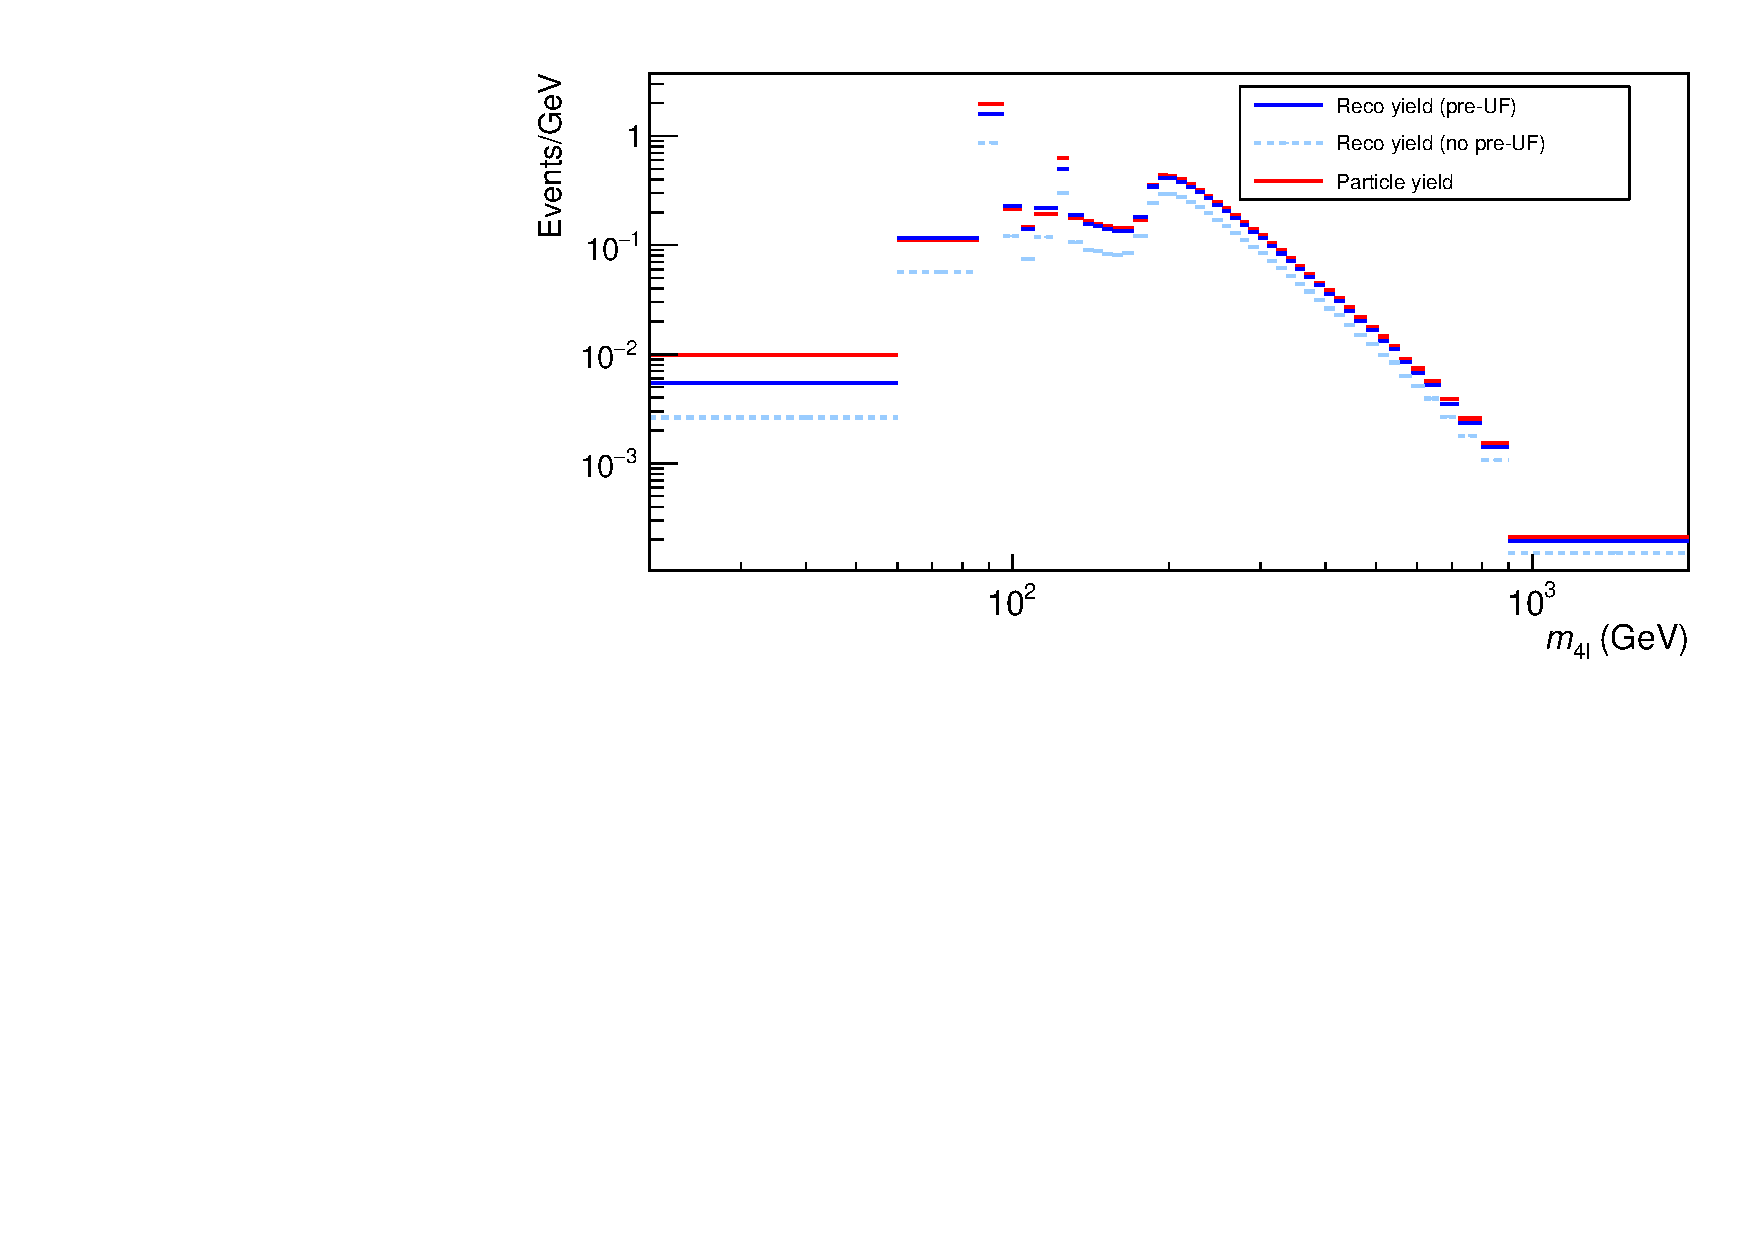
\includegraphics[width=.99\textwidth]{Figures/m4l/UnfoldingStudies/v014_preUF_compare.pdf}\caption{}
    \end{subfigure}
        \begin{subfigure}{.79\textwidth}\centering
        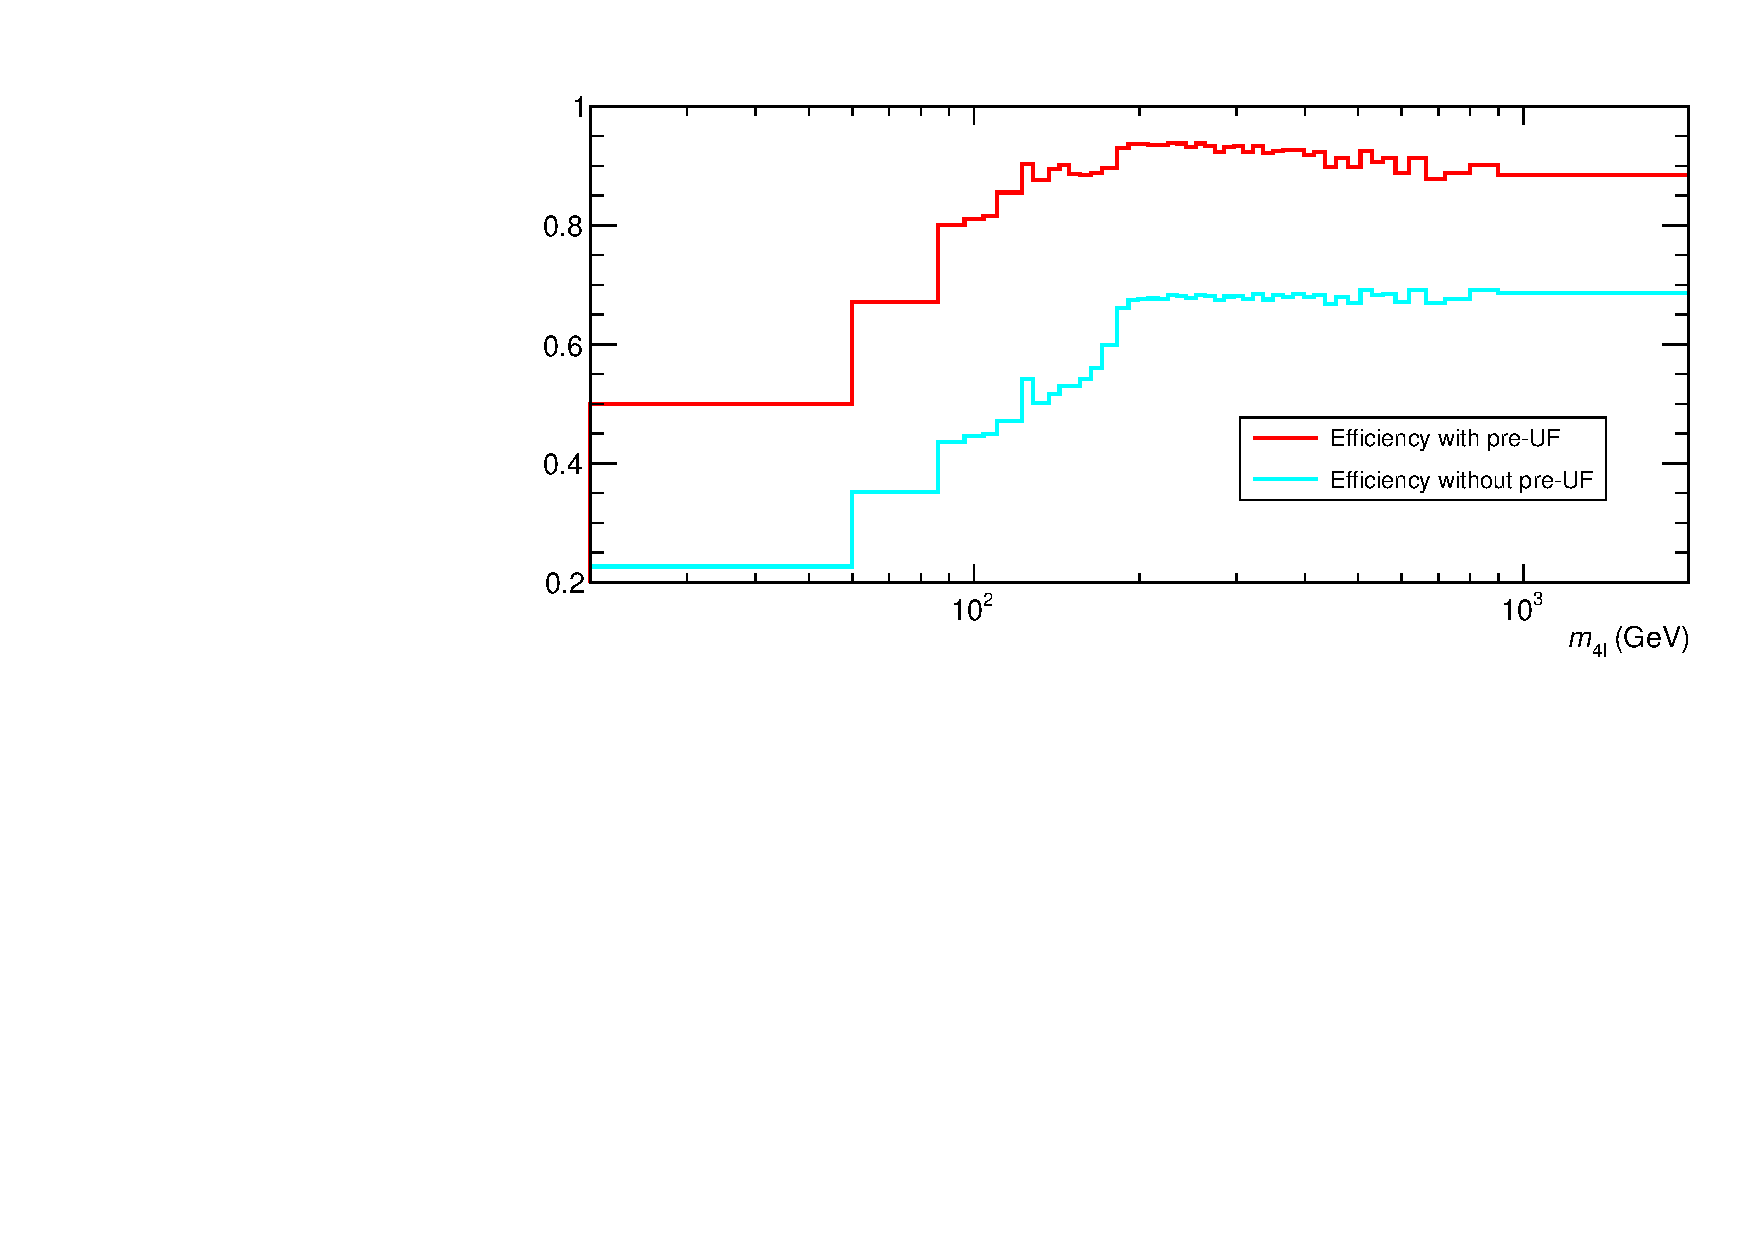
\includegraphics[width=.99\textwidth]{Figures/m4l/UnfoldingStudies/efficiency_preUF.pdf}\caption{}
    \end{subfigure}
    \caption{In the top panel is the effect of the pre-unfolding weights on the predicted detector level (also called reco level) yield, compared to the particle level yield. The bottom panel shows the reconstruction efficiency with and without application of the pre-unfolding weights. The pre-unfolding weights brings the detector yield closer to the particle yield, consequently the efficiency is much higher.}
    \label{fig:preUF}
\end{figure}

Figure \ref{fig:preUF} shows the detector yield from simulation with and without the application of the pre-unfolding weights, compared to the particle yield. It is readily apparent that the detector yield comes much closer to the particle yield when pre-unfolding weights are applied. In some cases, the detector yield surpasses the particle yield around the resonance peaks. This is attributed to bin migrations, and has negligible effects on the final unfolded result. Also shown is the efficiency correction with and without the pre-unfolding weights. In general, a significant increase in efficiency throughout the whole \mFourL{} spectrum, ranging from 10\% at low mass, up to 25\% at high mass. The conclusion drawn from these plots is that a large portion of the event inefficiency can be accounted for using per-lepton corrections, bringing the reconstructed and particle level yield closer to one another, and minimising the correction needed when unfolding.

\subsection{Unfolding iterations optimization}
\label{ssec:unfoldingiterations}
With the observable binnings defined and the pre-unfolding weights applied, the next step is to optimize the number of iterations used in the unfolding. As described in Section \ref{ssec:bayesianunfolding}, the iterative Bayesian approach to unfolding uses the Standard Model prediction as an initial prior and therefore has a dependence on it. Fewer numbers of iterations therefore correspond to a larger regularizaton bias on the unfolded result. Contrarily, increasing the number of iterations reduces the bias at the cost of a larger statistical uncertainty and results that are more prone to large bin-to-bin fluctuations. The rest of this section describes the metric used to balance these effects and converge on an optimal number of iterations.

First, one thousand toy distributions are generated from the Standard Model predicted yield at the detector level by drawing random Gaussian distributed values for each bin. Under the assumption that the SM accurately describes the underlying physics, each toy distribution represents a possible observation. The toy distributions are unfolded using the nominal unfolding method (Section \ref{subsec:unfmethod}). The bias of the unfolded toy result is defined using the migration matrix $M$, the unfolded yield of the toy $U_{j}$ , detector-level yield of the toy $R_i$, and the fiducial fraction $f_i$ as:
\begin{equation*}
  \text{Bias}_{\text{reco bin }i} = \frac{\sum\limits_{\text{truth bin }j} M_{ij} \times U_{j} - R_{i} \times f_{i} }{R_{i} \times f_{i}},
\end{equation*}
The bias significance of the toy is then be calculated in each bin as the ratio of the bias and the estimated statistical uncertainty of the unfolding procedure. This ratio is a comparison of the sizes of the two effects. 

Next, the bias significance of the one thousand toys are combined into a singular root-mean-square value in each bin. As a result, a metric indicating how significant the bias is expected to be across a range of toy datasets assuming an underlying SM physics is created. The number of iterations is chosen to be the smallest possible while maintaining a root-mean-square bias significance of 0.5 or below. This choice corresponds to a factor two suppresion of the bias compared to the statistical uncertainty. For the majority of distributions, three iterations of the unfolding comfortably satisfy this criteria, whilst for \mZOne-\mFourL, \dPhill-\mFourL{} and \dYPairs-\mFourL{} two iterations is sufficient. 
% The bias defined in this way is a measure of to which degree the individual toy is pulled towards the original standard model shape by the regularisation procedure in the unfolding. 
\subsection{Closure tests}
\label{ssec:closuretests}
\subsubsection{Monte Carlo closure tests}

As detailed in Section \ref{subsec:unfmethod}, the unfolding procedure uses a response matrix that has been derived from Standard Model Monte Carlo predictions. A simple test that can be performed to check the validity of the unfolding method is to use the same SM MC prediction at reconstruction level as pseudo-data, unfold it, and compare it to the truth level prediction. This is a self-consistency check, and should yield the trivial result that the unfolded pseudo-data be identical to the truth distribution. This is the full MC closure test, and acts as a sanity check for the unfolding procedure. The test is shown in Figure \ref{fig:fullMCclosure} for the inclusive \mFourL{} distribution. Full closure is achieved as the unfolded distribution and the particle-level distribution are identical. This is the case for all other distributions as well.

Another similar validation, the half MC closure test, is also performed. This time, the SM samples are divided in two sets A and B based on whether their tagged event number is odd or even. Set A is used to construct the fiducial fraction, reconstruction efficiency, and migration matrix, while set B is used as pseudo-data and unfolded with the inputs from the set A. The unfolded distribution of the set B is then compared to the true distribution of the set B. The statistical uncertainties on both sub-samples are evaluated via the bootstrap method~\cite{ATLAS_Bootsrap_2021}. Figure \ref{fig:halfMCclosure} shows the test result for the inclusive \mFourL{} spectrum. For this and all other distributions, closure is generally achieved within the statistical uncertainties in each bin, with no significant discrepancies. 

\begin{figure}
    \begin{subfigure}{.88\textwidth}\centering
        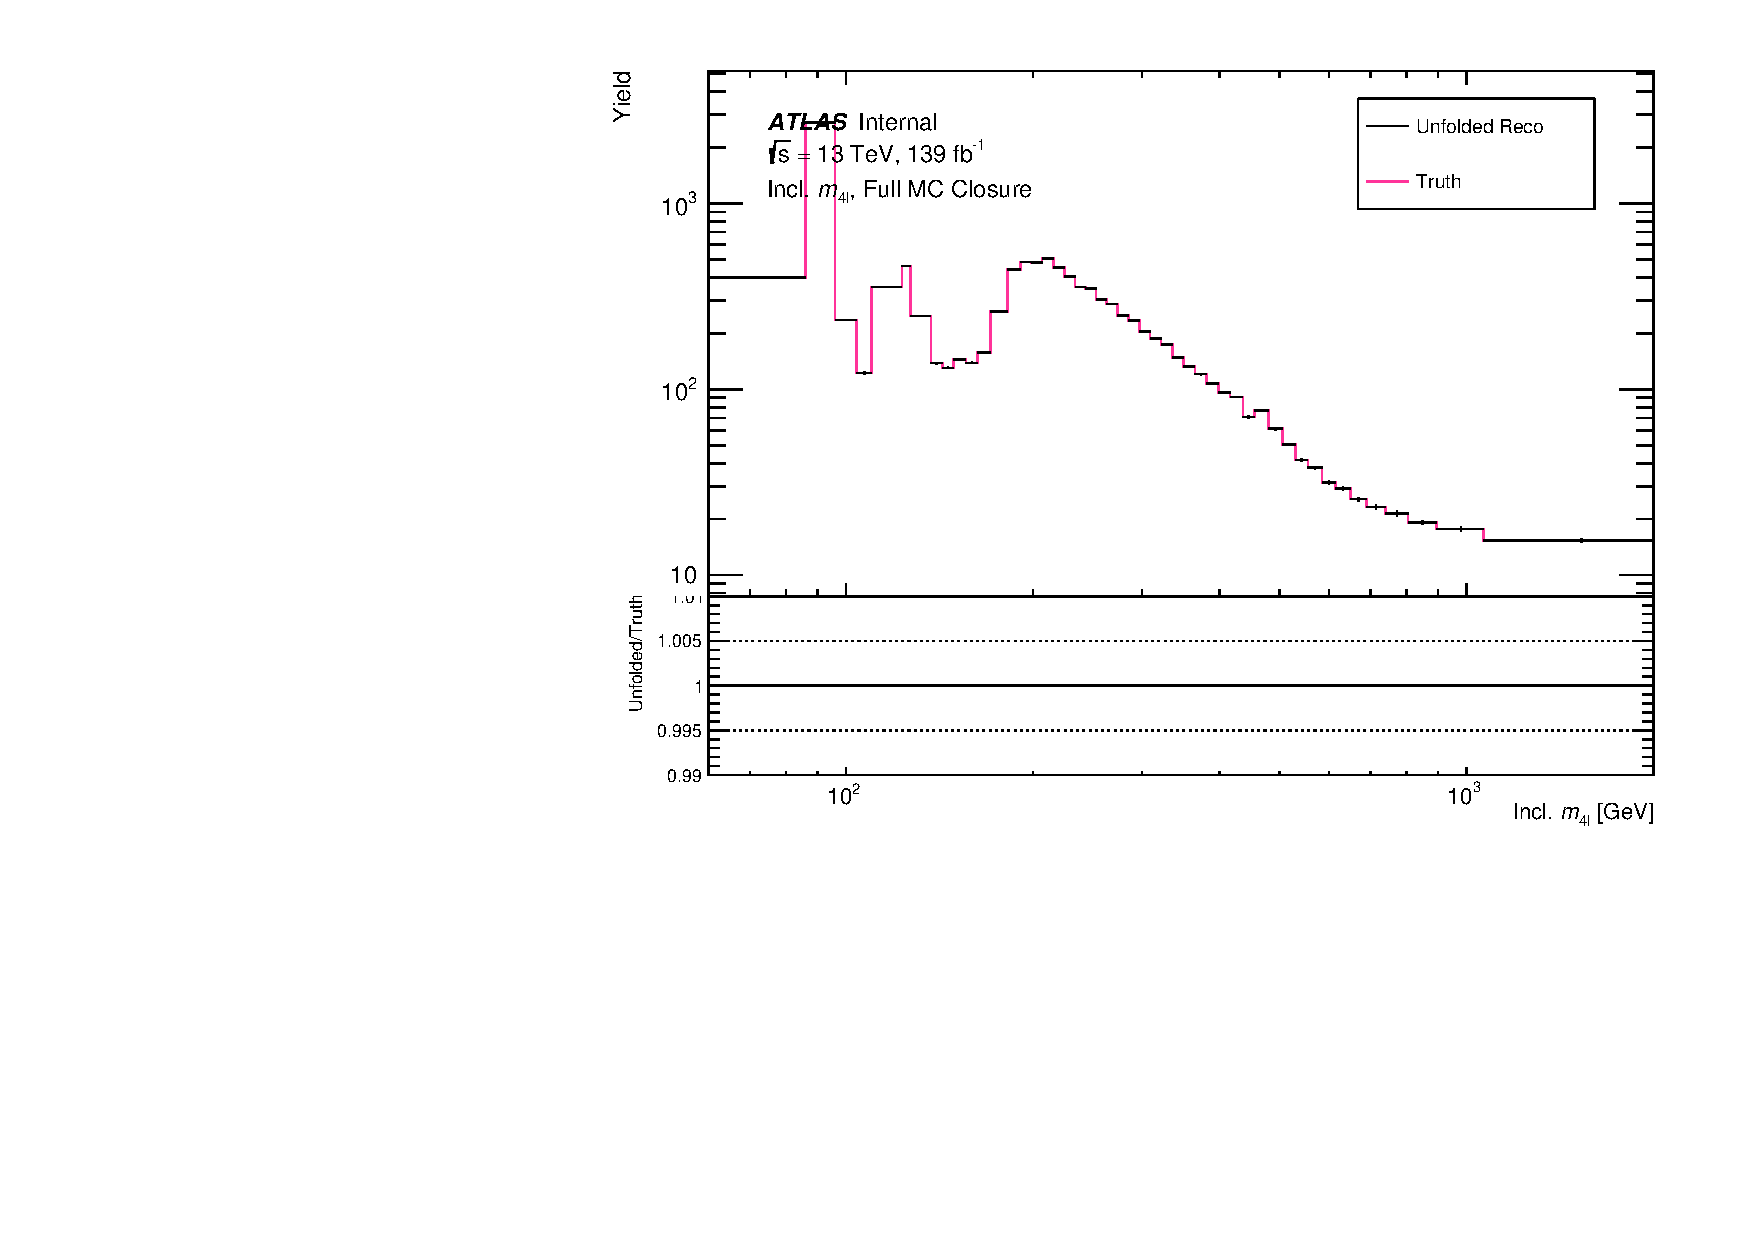
\includegraphics[width=0.90\linewidth]{Figures/m4l/MCClosure/FullMCClosure_inclm4l.pdf}\caption{}\label{fig:fullMCclosure}
    \end{subfigure}
        \begin{subfigure}{.8\textwidth}\centering
        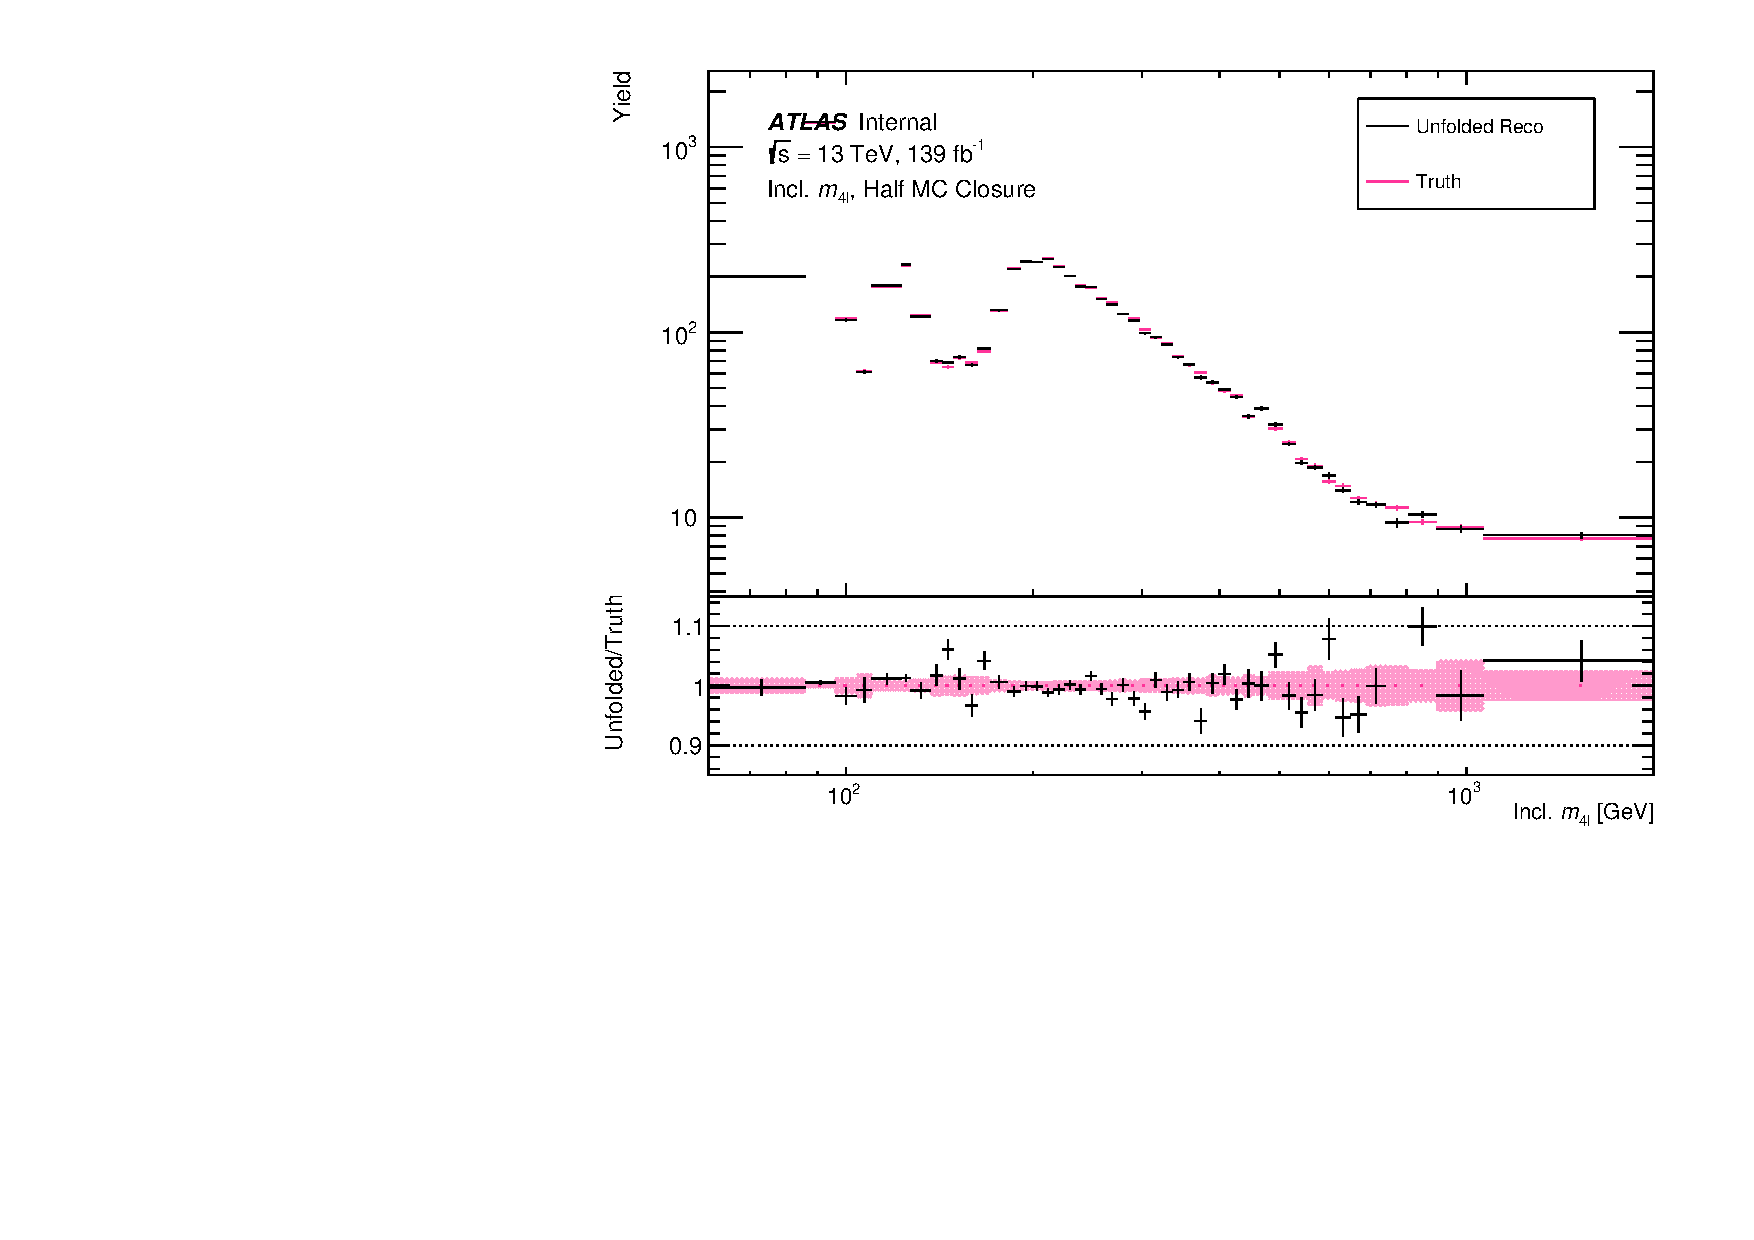
\includegraphics[width=0.99\linewidth]{Figures/m4l/MCClosure/HalfMCClosure_inclm4l.pdf}\caption{}\label{fig:halfMCclosure}
    \end{subfigure}
    \caption{Monte Carlo closure tests performed on all bins in the inclusive \mFourL{} distribution. The top figure uses the full MC to unfold itself. The bottom figure splits the MC in half, and uses one set to unfold the other. The pink hash in \ref{fig:halfMCclosure} is the MC statistical uncertainty. Closure is achieved in all bins.}
    \label{fig:MCclosure}
\end{figure}

\subsubsection{Data-driven closure tests}
\label{sssec:datadrivenclosure}
In order to assess the potential bias in the unfolding method, a data-driven closure test is performed separately for each measured distribution. For this test, a reweighting is conducted on the particle-level MC prediction such that the detector-level prediction represents more accurately the data. The function used for the reweighting is a smoothed function of the data to MC ratio. The reweighted prediction is used as pseudo-data and propagated through the nominal unfolding procedure. The difference between the reweighted particle-level prediction and the unfolded result in each bin is taken to be the systematic uncertainty of the unfolding method. The associated systematic uncertainty is below 0.3\% across the full mass range. For the double differential observables, the derived systematic uncertainties averaging much less than 1\% but reaching 3\% in a few bins. Overall, it remains subdominant compared to other sources of uncertainty.

\subsection{Injection studies}
\label{ssec:injectiontests}
Section \ref{ssec:closuretests} demonstrates that the unfolding procedure has closure when unfolding pseudo-data that agree with the Standard Model. Since the SM predictions themselves were used to derive the corrections and matrix used for unfolding, this is the expected case. The shape of real data is unknown, however, and may be different than the Standard Model prediction. Should the \mFourL{} spectrum be host to contributions that differ from the SM prediction, it is necessary to check that the unfolding procedure is nonetheless able to provide an accurate and unbiased particle-level result. In order to do this a number of injection tests were performed. The first step is to take the nominal SM prediction, and inject some amount of BSM signal into it. The reconstruction level yield of this modified sample is used as pseudo-data. It is run through the standard unfolding workflow in entirety, and compared to the particle level yield of the modified sample. Conceptually, this procedure is very similar to that of the Monte Carlo closure tests. 

A number of modifications were made to the nominal SM prediction, one set had the addition of a gluon-gluon fusion produced heavy Higgs boson with a mass of 300, 800, or \unit{1400}{\GeV} with either a narrow width or a width 15\% of its mass, and another set where the heavy Higgs was produced via vector-boson fusion. The \ggZZ process was also modified to have a larger event weight with respect to the SM prediction. These are described in full in Table \ref{tab:injectionsamples}. All of the models describe BSM scenarios with extremely large enhancements or resonances. 
\begin{table}[tbp]
    \begin{tabular}{ll}
        Injected samples \\
        \hline\\
         Gluon-gluon fusion (Narrow width)   & $m_{\text{res}}=$ 300, 800, 1400 GeV\\
        Gluon-gluon fusion (15\% width)      & $m_{\text{res}}=$ 300, 800, 1400 GeV \\
         Vector-boson fusion    & $m_{\text{res}}=$ 300, 800, 1400 GeV \\
         \hline \\ 
         \ggZZ Enhancement & $c$\timesnominal, $c$ = 1.1, 1.2, 1.5, 2, 5, 1\\
    \end{tabular}
  \caption{Modifications made to the nominal SM prediction for injection studies.}
  \label{tab:injectionsamples}
\end{table}

For each of the variations listed in Table \ref{tab:injectionsamples}, a range of cross-sections were injected and then unfolded with and without application of the pre-unfolding weights. In order to carve a more realistic scenario, one of the injected cross-sections for the heavy Higgs samples was set to be just within the two-sigma band of the data uncertainty. This was done by increasing the injected cross-section and calculating the $p$-value between the BSM prediction and the data until a $p$-value smaller than or equal to 0.05 is reached. This is the $p$-value corresponding to a two-sigma significance. The results from the injection tests corresponding to a two-sigma injected amount for all the gluon-gluon fusion BSM samples are shown in Figure~\ref{fig:m4l:injection}. The nominal SM prediction and the modified BSM + SM prediction at particle level are shown (SM truth and BSM truth respectively), along with two unfolded BSM distributions, one with pre-unfolding (pre-UF) weights applied and one without. The lower panel is the ratio of the unfolded BSM distribution to the true BSM distribution and is interpreted as the bias. 

Figure~\ref{fig:injection_6dot175fb_300w15} is also published in Reference~\cite{m4l2021_paper}. It shows the result of the injection test using a BSM model with a resonance mass of $m_{\mathrm{res}}=300~\GeV{}$ and width 15\% of the mass, with a cross-section of \unit{6.18}{\invfb}. Looking at the ratio panel, the bias goes up to 2.2\% without the application of the pre-unfolding weights (in green). With the weights applied, the bias is smaller and remains within a $\pm0.8\%$ range (in black). The same trend holds true for the rest of the 15\% width samples, see Figures~\ref{fig:injection_0dot862fb_800w15}-\ref{fig:injection_0dot4032fb_1400w15}. Application of the pre-unfolding weights tend to result in a smaller bias, especially for \unit{300}{\GeV} and \unit{800}{\GeV} resonances. For the highest resonance mass at \unit{1400}{\GeV}, the pre-unfolding has a notable effect only in the last \mFourL{} mass bin, where it reduces the bias from 10\% to 4\%.

The gluon-gluon fusion narrow-width heavy Higgs models' injection test results are presented in Figures~\ref{fig:injection_1dot24fb_300NW}-\ref{fig:injection_0dot19fb_1400NW}. The unfolding method is much more sensitive to, and therefore less robust to, the presence of narrow resonances. Here, the pre-unfolding is not as effective in mitigating the effects of the BSM signal. The differences between the unfolded BSM and the truth BSM, however, is still within 6\% bias for the \unit{300}{\GeV} and \unit{1400}{\GeV} resonance mass models. For the \unit{800}{\GeV} model this goes up to 16\%. In all cases, the bias is well within the total uncertainty in the corresponding \mFourL{} mass bin. Similar conclusions are drawn for the the narrow-width VBF samples. 

Lastly, the results from enhancing the \ggZZ component of the SM prediction are shown in Figures~\ref{fig:}-\ref{fig:}. The range of the enhancements vary starting from 1.1 times the nominal amount, to 10 times the nominal amount. Once again, the unfolded spectra are compared with and without the application of pre-unfolding weights. Looking at the bottom ratio pad, it is immediately evident from Figures~\ref{fig:}-\ref{fig:} that application of pre-unfolding weights leads to a smaller bias (i.e. a smaller difference between the true histogram and the unfolded histogram), especially at high mass. The unfolding procedure is very robust even for a \ggZZ enhancement ten times the SM amount; the bias for all bins are within 4\%.

\begin{figure}[htb]
    \begin{subfigure}{.49\textwidth}\centering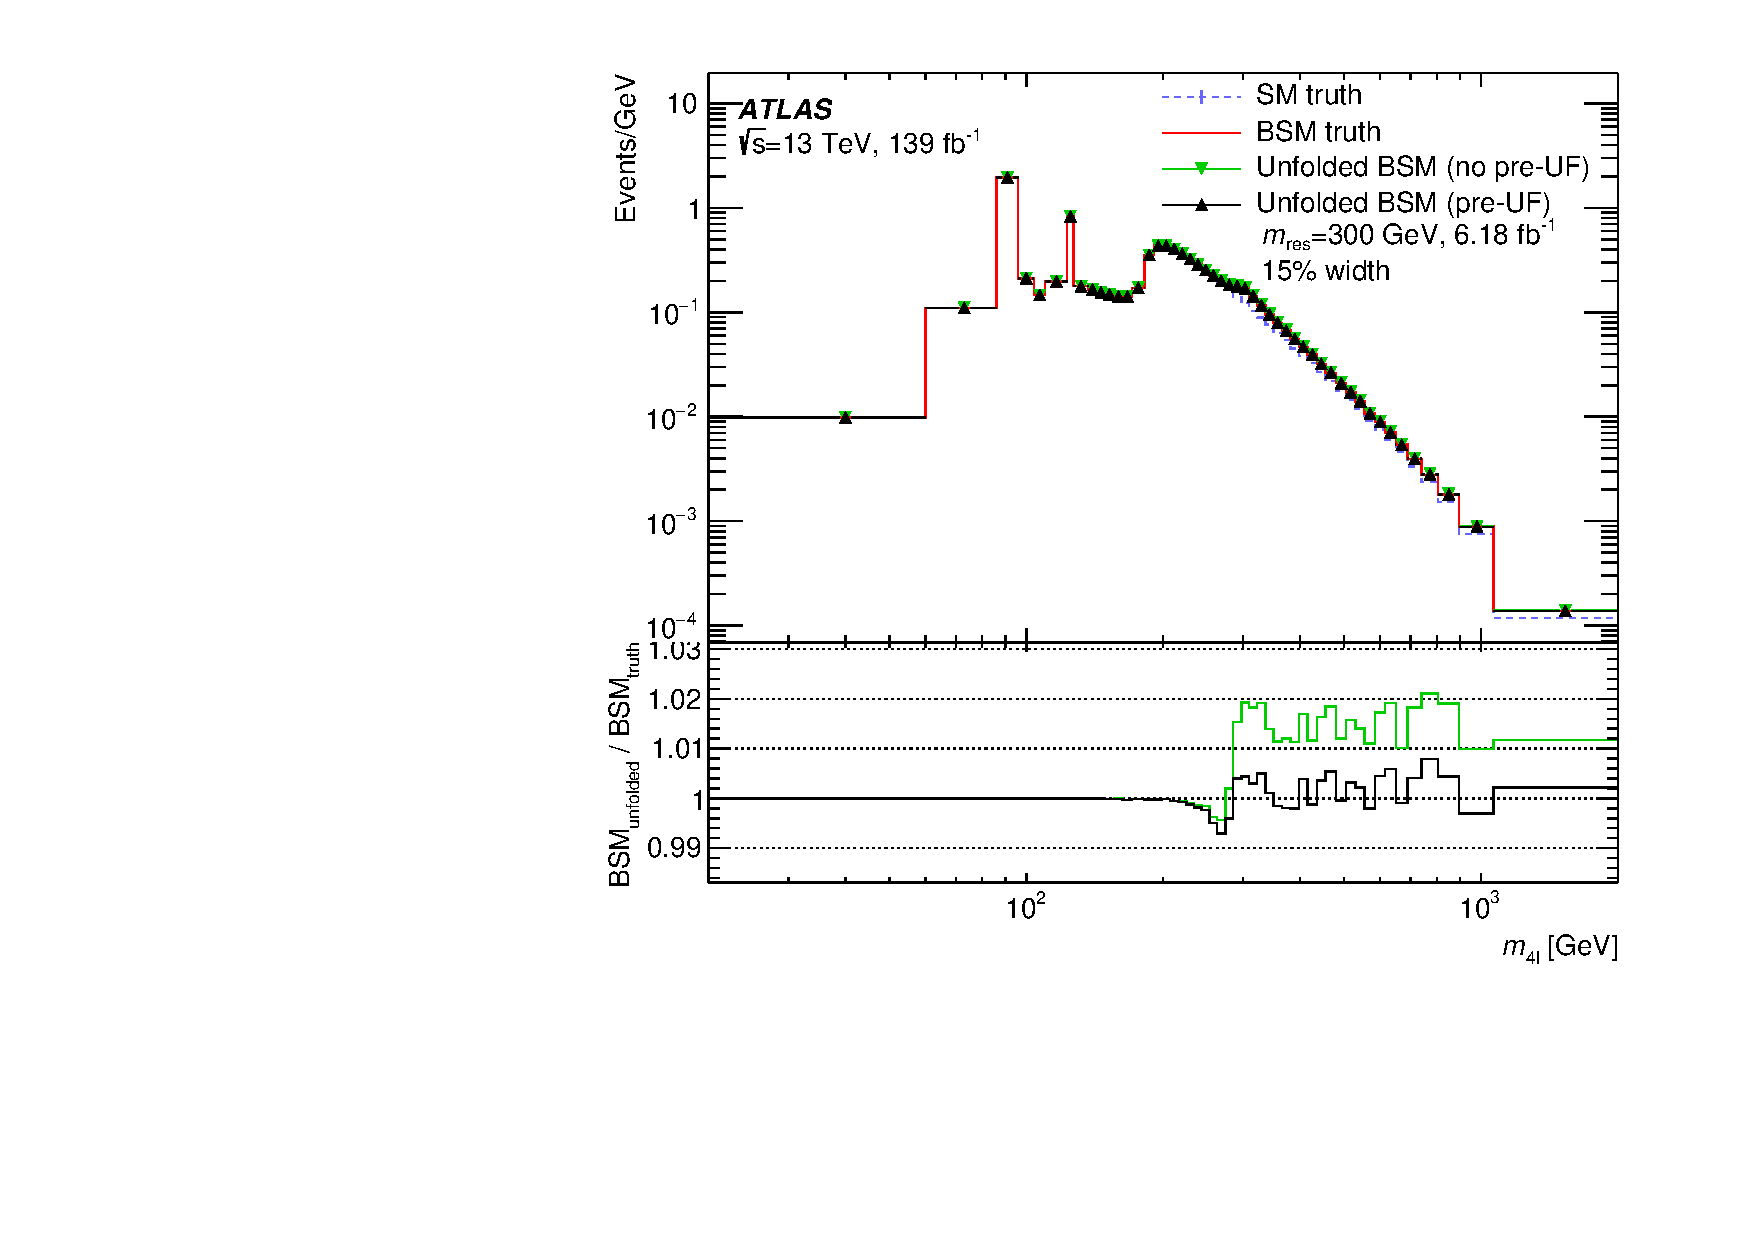
\includegraphics[width = 0.95\textwidth]{Figures/m4l/InjectionTests/6dot175fb_300w15_injection.pdf}\caption{}\label{fig:injection_6dot175fb_300w15}\end{subfigure}
    \begin{subfigure}{.49\textwidth}\centering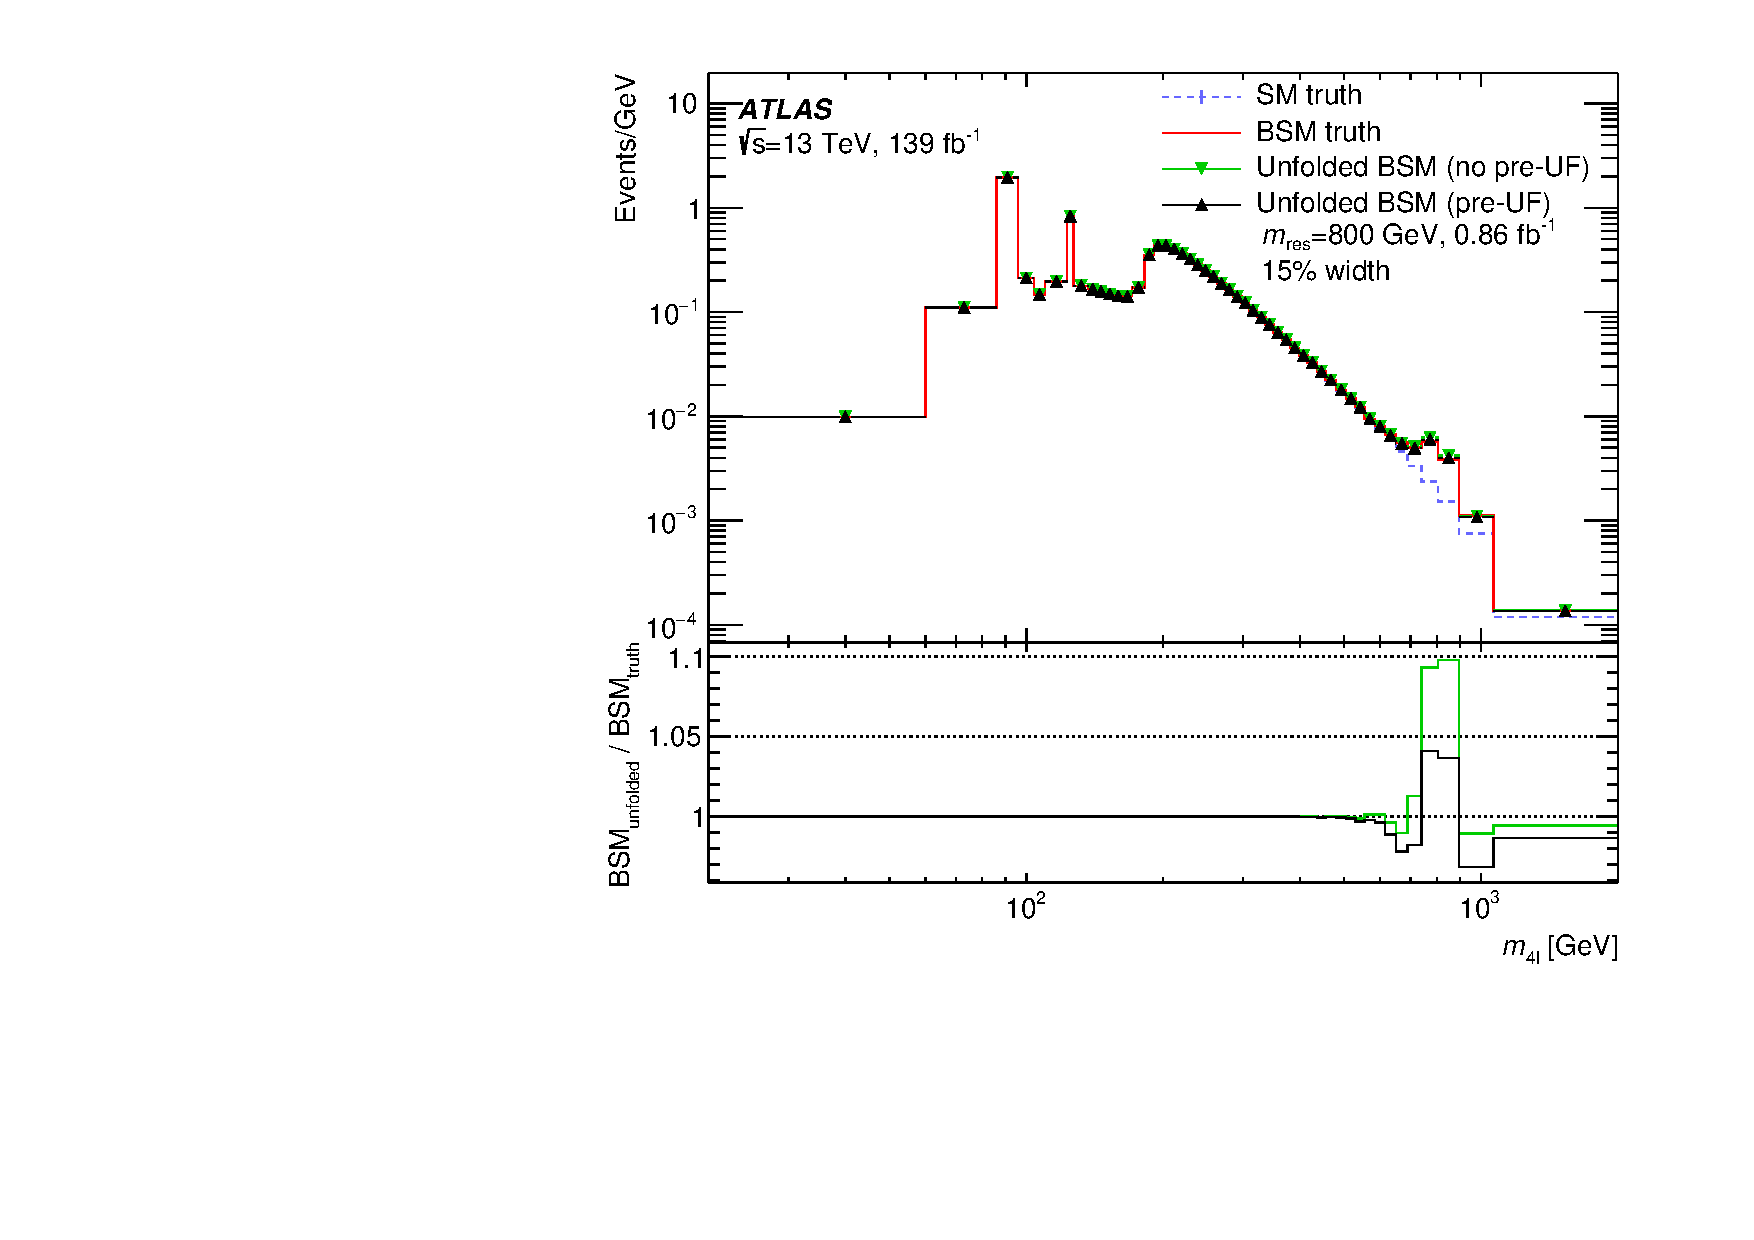
\includegraphics[width = 0.95\textwidth]{Figures/m4l/InjectionTests/0dot862fb_800w15_injection.pdf}\caption{}\label{fig:injection_0dot862fb_800w15}\end{subfigure}
    \begin{subfigure}{.49\textwidth}\centering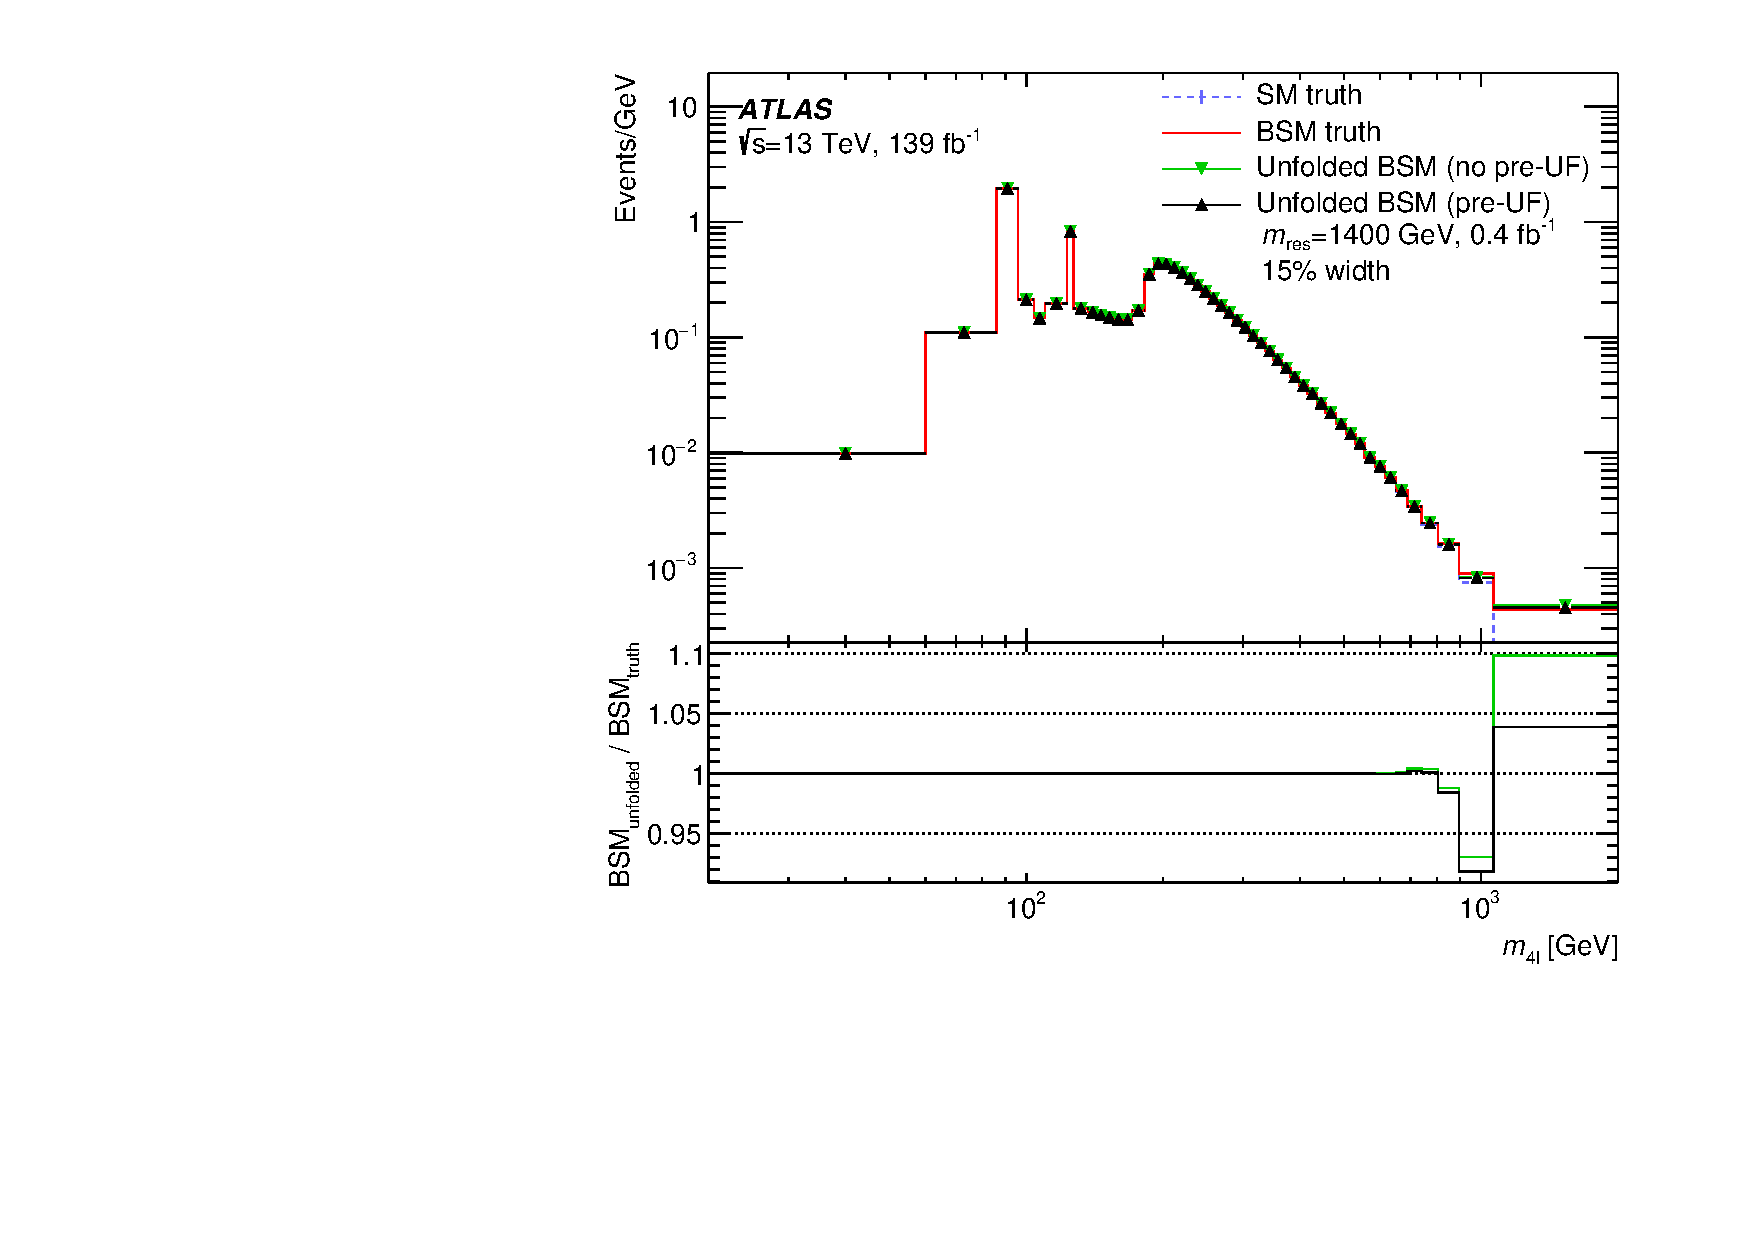
\includegraphics[width = 0.95\textwidth]{Figures/m4l/InjectionTests/0dot4032fb_1400w15_injection.pdf}\caption{}\label{fig:injection_0dot4032fb_1400w15}\end{subfigure}
    \begin{subfigure}{.49\textwidth}\centering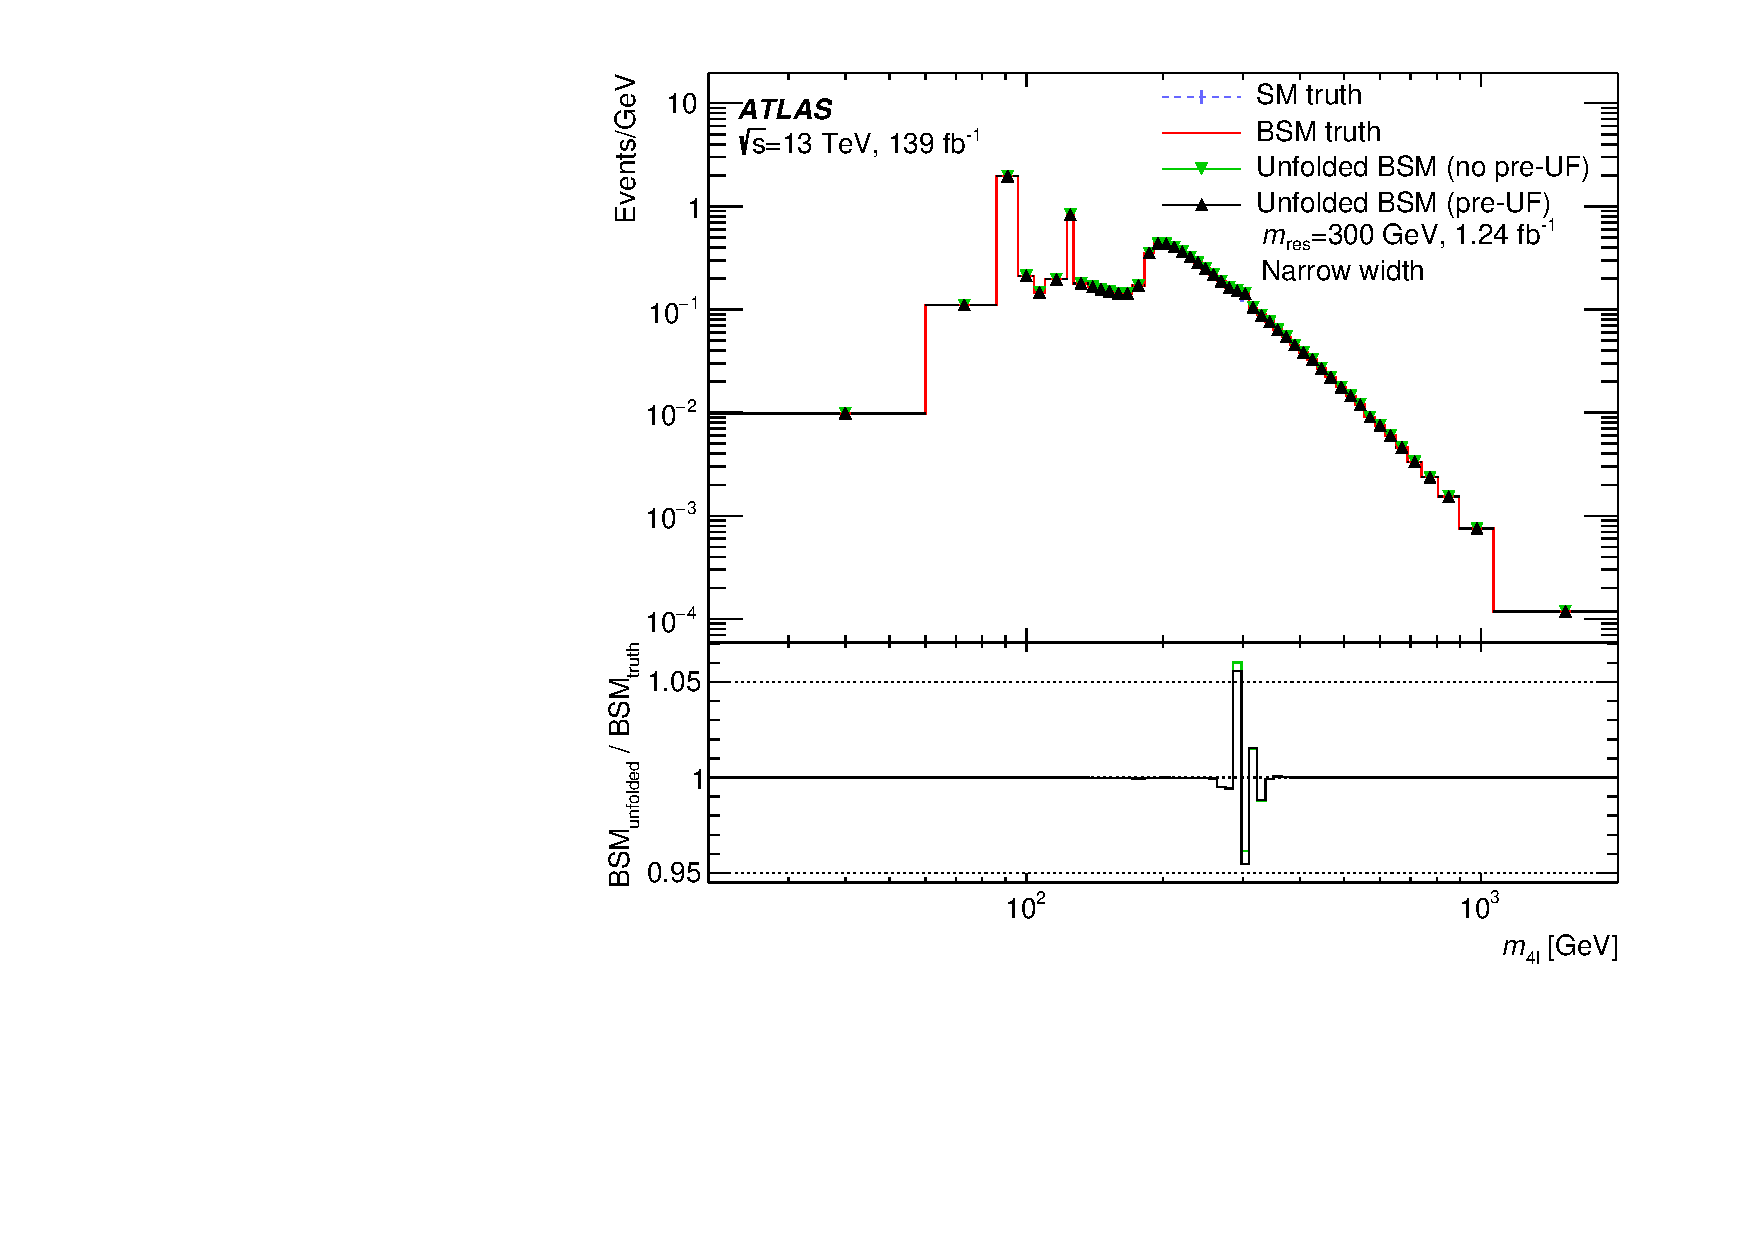
\includegraphics[width = 0.95\textwidth]{Figures/m4l/InjectionTests/1dot24fb_300NW_injection.pdf}\caption{}l\label{fig:injection_1dot24fb_300NW}\end{subfigure}
    \begin{subfigure}{.49\textwidth}\centering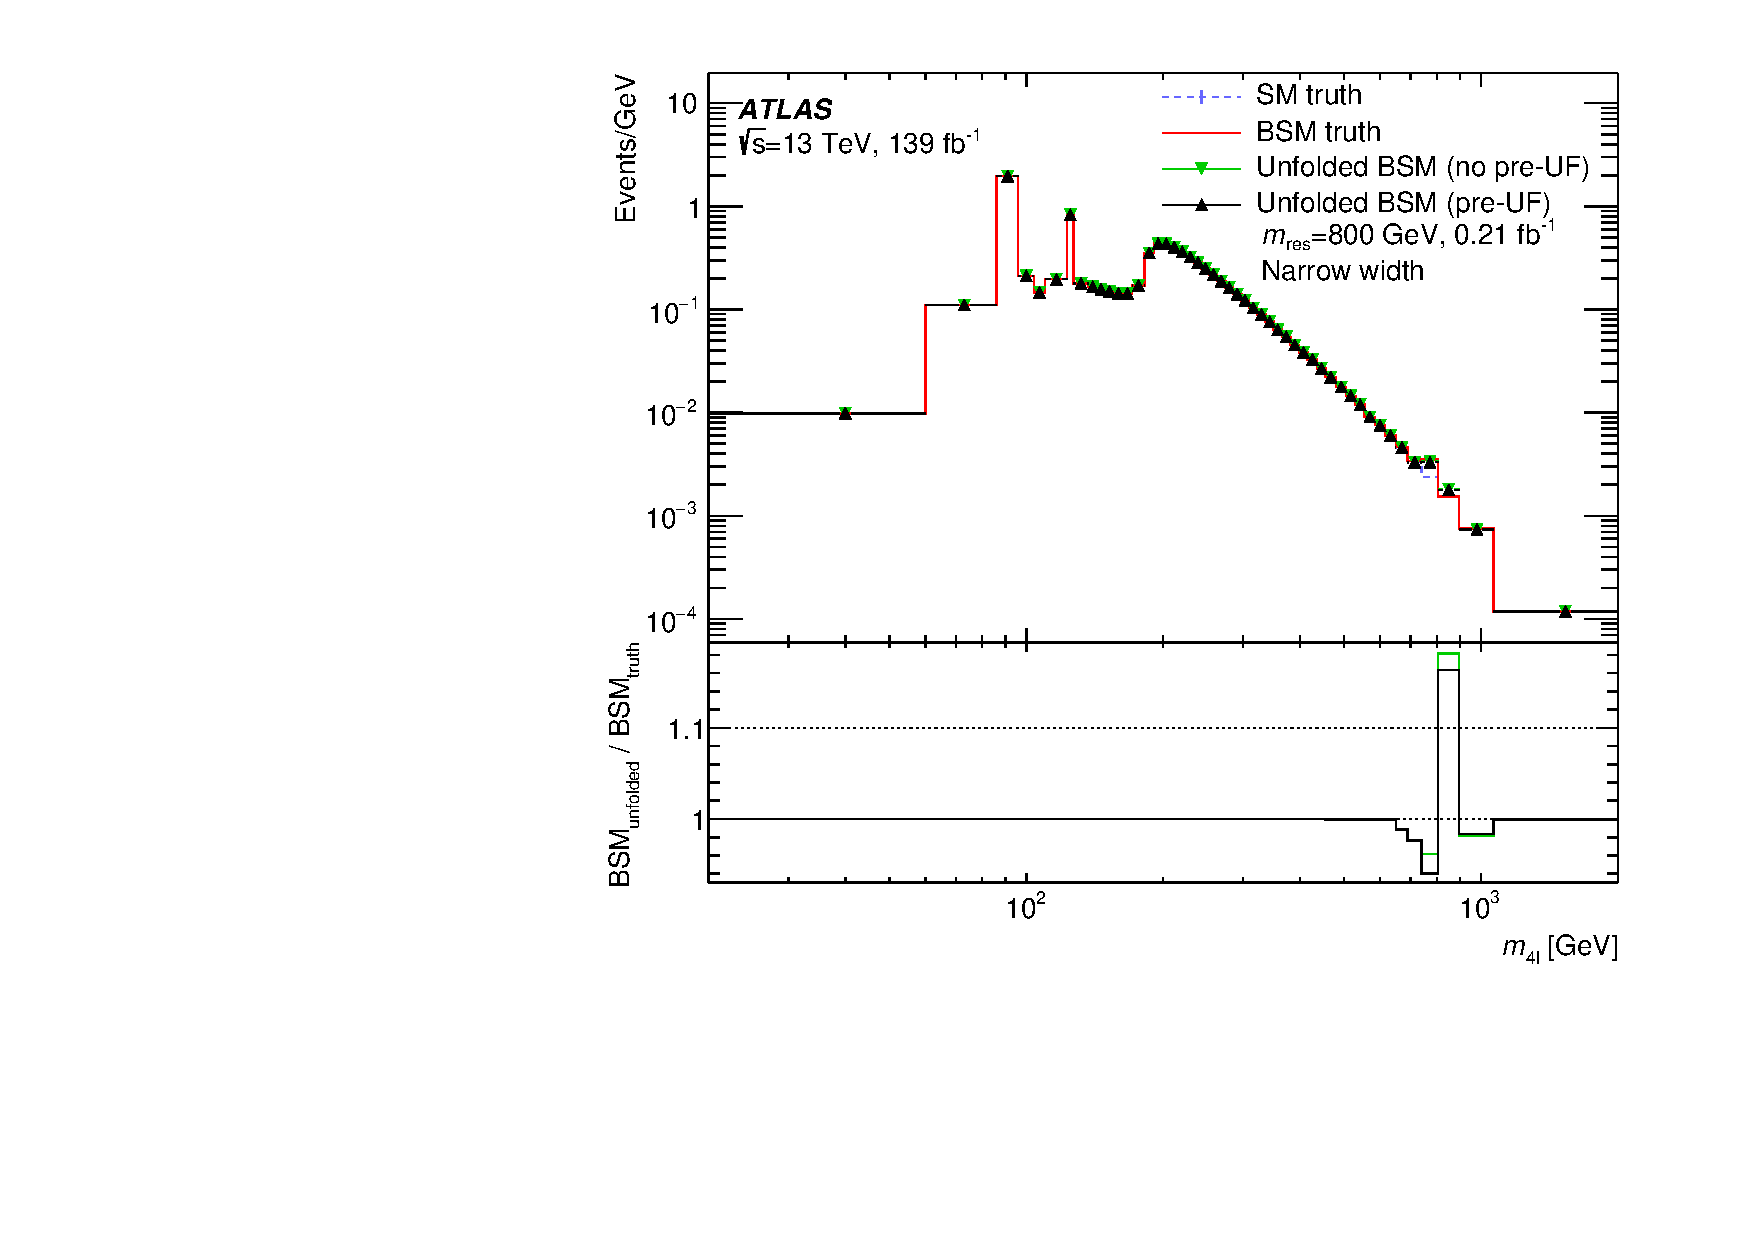
\includegraphics[width = 0.95\textwidth]{Figures/m4l/InjectionTests/0dot212fb_800NW_injection.pdf}\caption{}\end{subfigure}
    \begin{subfigure}{.49\textwidth}\centering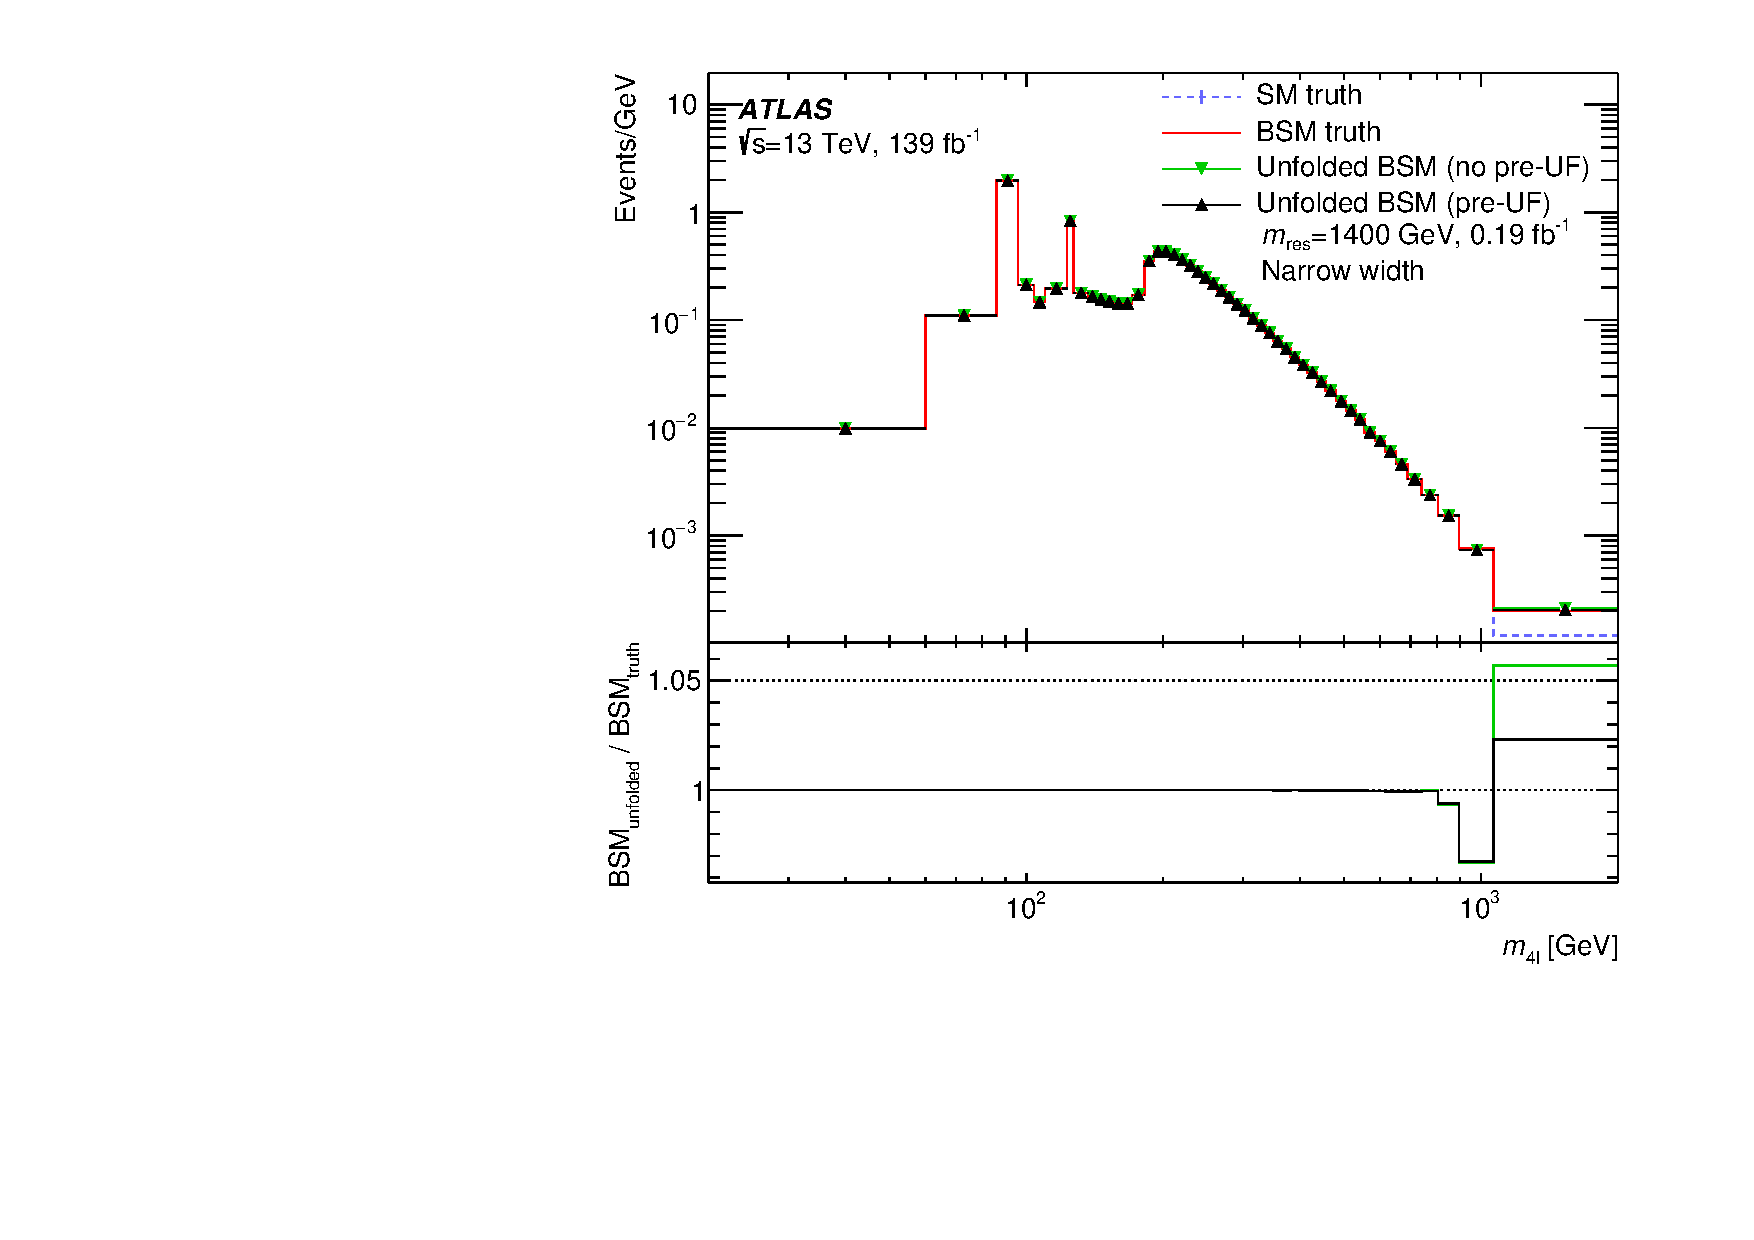
\includegraphics[width = 0.95\textwidth]{Figures/m4l/InjectionTests/0dot19fb_1400NW_injection.pdf}\caption{}\label{fig:injection_0dot19fb_1400NW}\end{subfigure}
    \caption{This figure shows the results of the BSM signal injection studies performed on the \mFourL{} distribution. Six BSM models are considered, with resonance masses at 300~\GeV, 800~\GeV, and 1400~\GeV, and with narrow widths or a width 15\% of the resonance mass. The cross-sections correspond to a $2\sigma$ signal significant with respect to the data uncertainty. Two unfolded distributions are shown with and without pre-unfolding (pre-UF) weights applied. The bottom panel shows the size of the bias.}
    \label{fig:m4l:injection}
\end{figure}